\documentclass[a4paper, 12pt]{report}
\usepackage{amssymb}  % Symbol collection
\usepackage[toc,page]{appendix}
\usepackage[english]{babel}  % Multilingual support
\usepackage{cite}  % Improved citation handling
\usepackage{enumitem}  % Control layout of itemize, enumerate, description
\usepackage{ellipsis}
\usepackage{fancyhdr}  % Extensive control of page headers and footers
\usepackage[Bjornstrup]{fncychap}  % Seven predefined chapter heading styles
\usepackage{hyperref}  % Extensive support for hypertext
\usepackage{indentfirst}  % Indent first paragraph after section header
\usepackage[utf8x]{inputenc}  % Accept different input encodings
\usepackage{lipsum}
\usepackage{listings}  % Typeset source code listings
\usepackage{setspace}  % Set space between lines
\usepackage{svg}  % Include and extract SVG pictures
\setlength{\marginparwidth}{2cm}
\usepackage{textcomp}
\usepackage{todonotes}
\usepackage{ucs}  % Extended UTF-8 input encoding support
\usepackage{url}  % Verbatim with URL-sensitive line breaks
\usepackage{xcolor}

\definecolor{codegreen}{rgb}{0,0.6,0}
\definecolor{codegray}{rgb}{0.5,0.5,0.5}
\definecolor{codepurple}{rgb}{0.58,0,0.82}
\definecolor{backcolour}{rgb}{0.95,0.95,0.92}

\lstdefinestyle{mystyle}{
    backgroundcolor=\color{backcolour},
    commentstyle=\color{codegreen},
    keywordstyle=\color{magenta},
    numberstyle=\tiny\color{codegray},
    stringstyle=\color{codepurple},
    basicstyle=\ttfamily\scriptsize,
    breakatwhitespace=false,
    breaklines=true,
    captionpos=b,
    keepspaces=true,
    numbers=left,
    numbersep=5pt,
    showspaces=false,
    showstringspaces=false,
    showtabs=false,
    tabsize=2,
    escapeinside={|*}{*|},
    upquote=true
}

\lstset{style=mystyle}

\author{Diego Russo}
\title{Master Degree Thesis}
\date{2021\-02\-23}

\frenchspacing

\hypersetup{
    colorlinks=true,
    linkcolor=blue,
    filecolor=magenta,
    urlcolor=cyan,
    pdfpagemode=FullScreen,
}

\begin{document}

    \begin{titlepage}
    \begin{center}
        \textbf{\Large UNIVERSITY OF PERUGIA}\\
        \textbf{UNIVERSITÀ DI PERUGIA}
        \vspace{0.5cm}

        \scshape{Faculty of Mathematical, Physical and Natural Sciences}\\
        \scshape{Facoltà di Scienze Matematiche, Fisiche e Naturali}
        \vspace{0.5cm}

        \scshape{Department of Mathematics and Computer Science}\\
        \scshape{Dipartimento di Matematica ed Informatica}

        \rule[1mm]{\textwidth}{0.2mm}
        \vspace{0.5cm}

        \begin{Large}Master Degree in Computer Science\end{Large}\\
        Laurea specialistica in Informatica
        \vspace{0.5cm}

        \begin{figure}[htbp]
            \begin{center}
                \includesvg[width=3cm]{images/unipg_logo.svg}
                
\includegraphics[width=3cm]{images/ssmmffnn_logo.jpg}\\
                
\includegraphics[width=3cm]{images/dmi_logo.png}
            \end{center}
        \end{figure}

        Master Degree Thesis:\\
        \vspace{0.5cm}
        \textbf{\LARGE Pruning with Heuristic}\\
        \vspace{0.3cm}
        Pruning a neural network with custom heuristic\\
        \vspace{1.5cm}

        \textbf{Author:} \hfill \textbf{Supervisors:}\\
        \textit{Diego Russo, 231423} \hfill \textit{Prof.\ Alfredo Milani}\\
        \textit{me@diegor.it} \hfill \textit{PhD.\ Anton Katchaktou}

        \rule[1mm]{\textwidth}{0.2mm}
        \small{Academic Year 2020/2021}
    \end{center}
\end{titlepage}

    \pagenumbering{arabic}
    \pagestyle{fancy}
    \rhead{}
    \tableofcontents{}
    \listoffigures{}
    \lstlistoflistings{}

    \thispagestyle{empty}

\begin{flushright}
    {\Huge\textit{``Now is better than never.''}}
    \linebreak
    \linebreak
    from ``The Zen of Python''
\end{flushright}

\clearpage

\thispagestyle{empty}

This thesis represents the end of a long journey started more than a decade
ago. Studying part-time has not been easy but it is definitively doable if one
has the right amount of perseverance, patience and determination: when I
enrolled to the master's degree I was already working as software developer and
I have been working since then.

\medskip

It has been a bumpy ride, full of unexpected turns of events which slowed
down the progress of my studies but at the same time they contributed to my
personal and professional life and they brought me where I am now: 2 more
spoken languages, new home country, new culture, new experiences, plenty of
working experience and, the most important, working on AI/ML field, a
long-awaited move.

I have always seen the master course as way to learn new things (even from the
``boring'' topics), to improve myself and to keep my mind in constant training.
Although stressful, and sometimes hard, I would do it again.

\medskip

This has been possible thanks to the support of many people who in a way or
another have helped me to go through difficult times.

First of all, to my family who has always believed and trusted me: their
support has been vital to get to the point where I am today.

My girlfriend Carmen who unconditionally has supported me during the last few
years for the final sprint of exams and thesis. Gracias mi amor!

Friends and people who, even with small words or actions, have given me the
strength to continue and to finish this journey.

\medskip

All the professors who, during all these years, have understood my working
abroad situation demonstrating flexibility and accommodating my needs.
Amongst them, a special thanks to Professor Alfredo Milani, the supervisor of
this thesis.

\medskip

Last but not least, a huge thank you to my employer Arm Ltd. They have been
very supportive with my studies during all these years allowing me extra days
whenever I needed to sit exams and for allowing me to work part-time during my
final sprint.

Within Arm, I would like to thank my current line manager and supervisor of
this thesis, Anton Kachatkou: his support has been fundamental for the
execution of this work. Anton supported and helped me to get the right
approvals within Arm, IP reviewed every single word/code of this thesis and
spent some of his time to discuss about this work.

I also wish to thank my team members, Mohamed Nour Abouelseoud, Ruomei Yan and
Johan Gras for reviewing my code and helping with experiments.

After all, it is a team effort, and the excellent results of this thesis are
because of everyone's contribution.

\medskip

Thank you all.

\clearpage

    \begin{abstract}
In the last decade Deep Learning has had a incredible success due to the
increasing availability of big data and the decreasing cost of compute power.
The research has been massive in all fields around Deep Learning: from new
network models to solve different problems to optimizations of such models
for deployment to edge devices with limited resources.
With almost 100 papers in the literature, pruning is amongst these techniques
with the aim to optimize the models to be more power and memory efficient while
having no or little drop in the accuracy.
This thesis shows a specific pruning technique: layers of a network model are
pruned based on a heuristic whilst respecting the target sparsity of the
network model.
After explaining the theory behind this approach, the code is explained and
applied to a simple MNIST based network model using TensorFlow Model
Optimization.
The ending chapter shows results of experiments running on MobileNet v1
architecture using CIRAF10 and ImageNet 2012 as datasets.
\todo{Add experiments results}
\end{abstract}
    \chapter{Introduction}\label{ch:introduction}
In the recent years we have been witnessing an incredible increase of
Artificial Intelligence (AI) applications and services.
Machine Learning (ML) and Deep Learning (DL) have been outperforming other
classical AI algorithms in many fields, like face recognition and natural
language processing.

This has been possible thanks to the explosion of data availability and compute
power, both needed and essential for ``training'' these neural networks.
Once the neural network has been trained, it can be used for the target that it
has been trained for: this phase is called ``inference''.
In \autoref{sec:training} I explain more in details these phases and what lies
in between.

Applications that requires some intelligence are computation intensive
demanding CPU, GPU, memory hence power out of the device and this makes the
application not always available to the end user.
In the last years the performance of these devices has been getting better and
better but still not sufficient for all more compute intensive applications.

The solution is to have a centralised data management and processing
(see~\ref{fig:centralised_intelligence}): the device collects data, send the
data to the cloud for processing and it receives back a response to their
request. This is called \textbf{centralised intelligence}.
Although this design is the basis of many applications, it presents some
drawbacks:
\begin{itemize}
    \item \textbf{amount of data}: the data generated by the device is sent to
        the cloud for processing. The amount of this data is not trivial and
        this could put under stress communication channels.
    \item \textbf{persistent connection}: in order to have a working
        application a persistent network connection between the device and the
        cloud computing is required.
    \item \textbf{real-time}: some applications cannot function properly when
        in presence of latency introduced by the communication between the
        device and cloud and any delay in processing the request by the cloud.
    \item \textbf{data privacy}: the device might send personal data to the
        cloud exposing privacy issues in case of hacking of leaking of
        information from the cloud provide.
\end{itemize}

\begin{figure}[ht]
    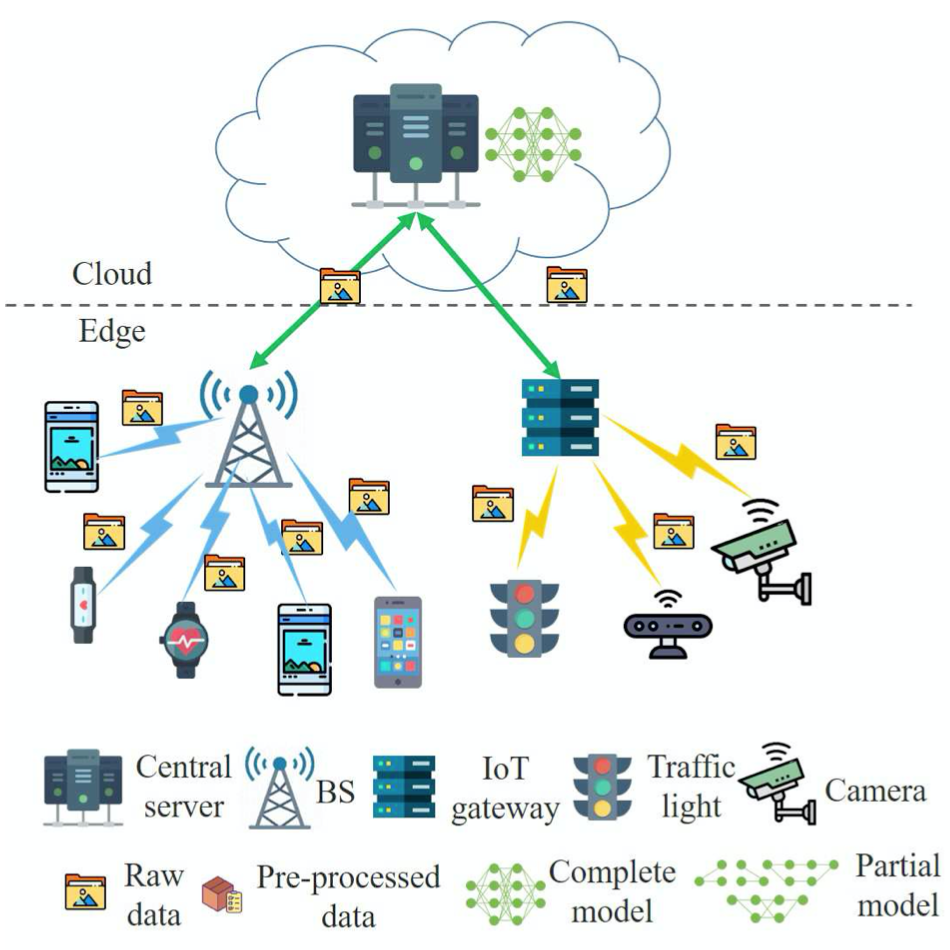
\includegraphics[width=10cm]{images/introduction/centralised_intelligence.png}
    \centering
    \caption{Centralised Intelligence}\label{fig:centralised_intelligence}
\end{figure}

In order to overcome to the above issues, a different approach is needed where
the data processing is not centralised but distributed closer where it is
generated: this different approach is called \textbf{edge computing},
Computing, storage and networking resources are located at the edge of the
network (IoT gateways, routers, etc\ldots) whilst end devices like mobile
phones and IoT devices request services from edge servers are called edge
devices.
It is easy to understand how this approach can address some of the issues in
the centralised intelligence: low latency between edge devices and edge servers
and data exchange and data privacy are some how mitigated.
It is worth noticing that edge computing is not a replacement for cloud
computing. On the contrary, it complements cloud computing and both are
targeting different kind of applications.

If we push a little more the design, the basis of edge computing combined with
AI creates what is called
\textbf{edge or mobile intelligence} (see~\ref{fig:edge_intelligence}).

This means that the data collection, caching, processing and analysis happens
on the device where the data is generated.
With this model latency, data privacy, network load and communication are all
contained and improved, giving a better experience to the end user and making
the application more reliable.

\begin{figure}[ht]
    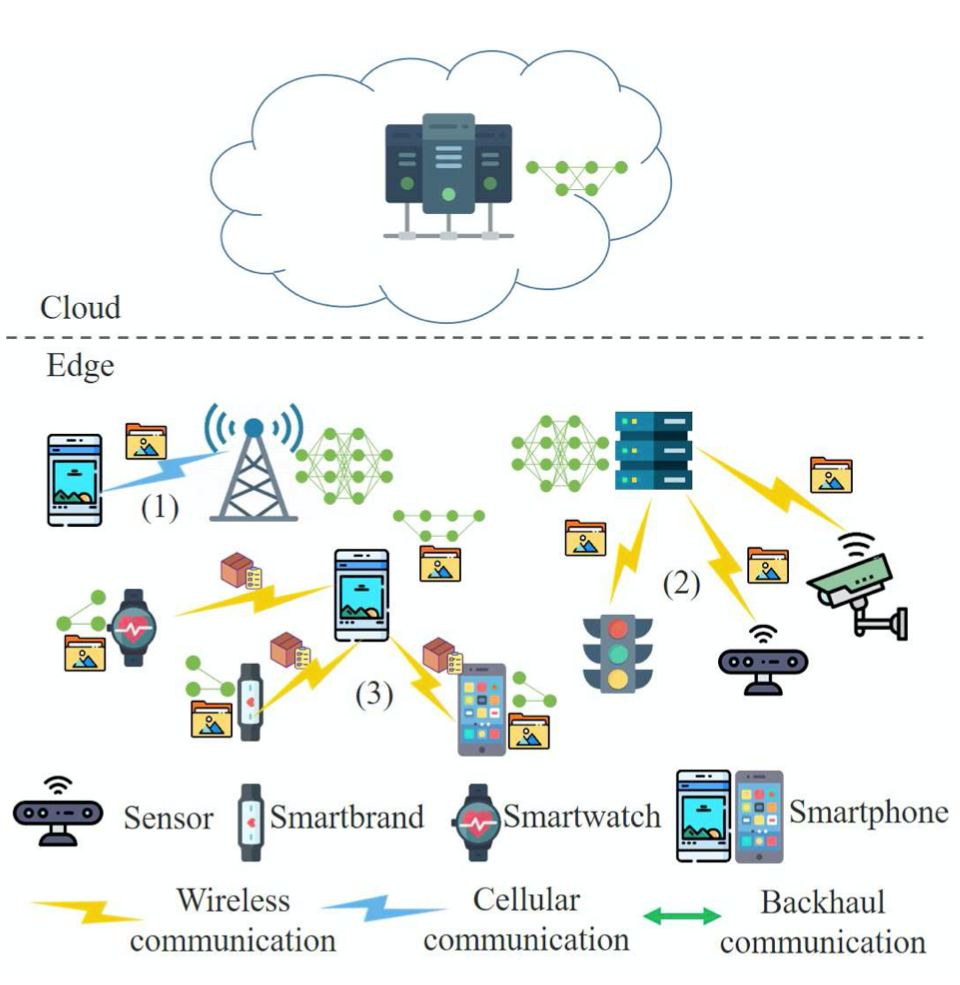
\includegraphics[width=10cm]{images/introduction/edge_intelligence.png}
    \centering
    \caption{Edge Intelligence}\label{fig:edge_intelligence}
\end{figure}

With more powerful end devices we start having edge intelligence applications
in our pockets like smart suggestions on the keyboards based on the context of
the text, photos application with integrated face recognition (note: no
personal data is sent to the cloud) based on contacts stored on the mobile and
voice recognition commands for offline translation and on mobile actions.
Other examples are also self-driving cars, real-time applications and medical
devices but also noise cancellation on video call application like Microsoft
Teams. Interestingly enough, as counter example Google Meet uses its model on
the cloud leveraging Google TPU infrastructure.

In this thesis I focus mainly on the \textbf{edge inference} (~\ref{fig:edge_inference})
and specifically how the models can be optimised in order to reduce memory
footprint, size and compression without losing any accuracy in the prediction.

\begin{figure}[ht]
    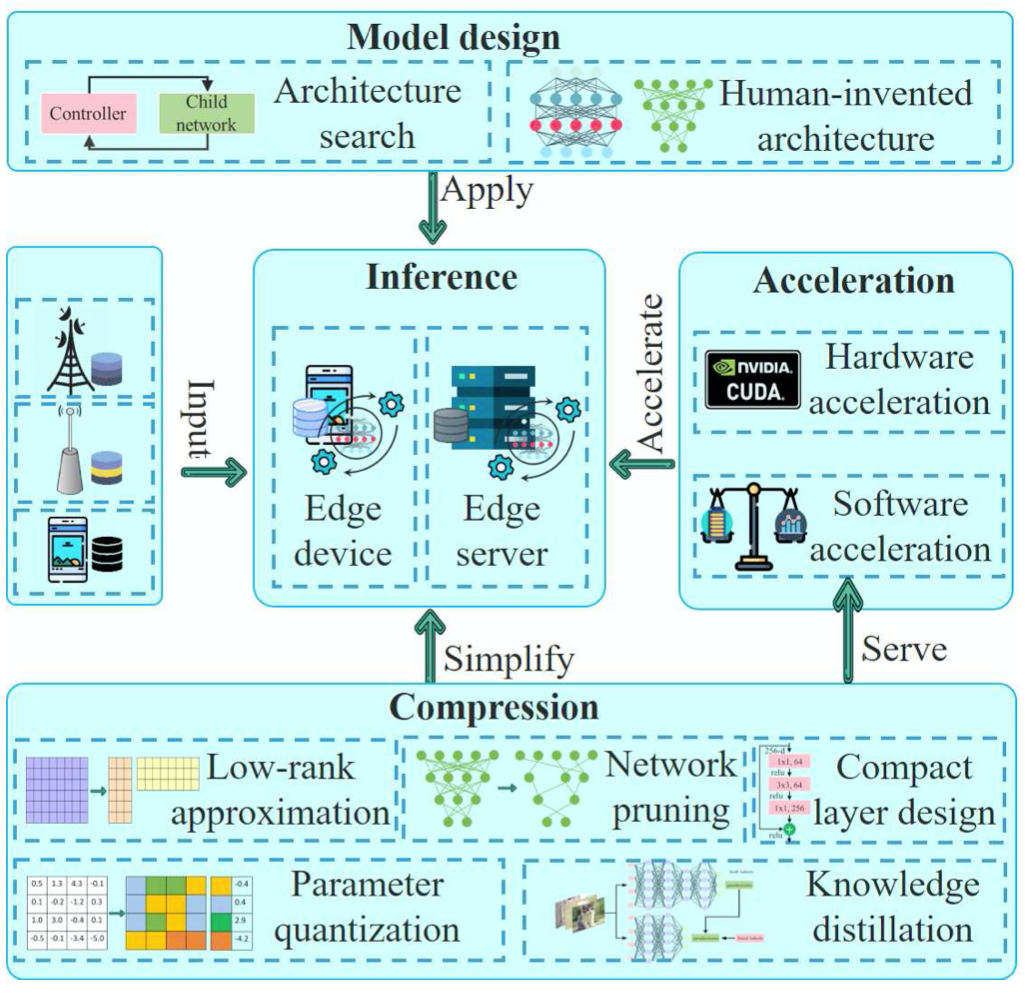
\includegraphics[width=10cm]{images/introduction/edge_inference.png}
    \centering
    \caption{Edge Inference}\label{fig:edge_inference}
\end{figure}

Edge inference is the final step of a model life cycle where the trained model
is used to infer new and unseen data via a forward pass of the neural network.
This step happens on the edge device and it presents some challenges due to the
limited amount of compute power and memory on the device itself.

In order to work correctly end efficiently the model needs to go through a
series of optimisations that decreases the power/memory consumption and latency
whilst maintaining the accuracy at acceptable levels \- ideally without
incurring in any decrease.

As the figure~\ref{fig:edge_inference} shows, there are different techniques
that it can be used to optimise models for edge inference. These are:
\begin{itemize}
    \item \textbf{Model design}: let the machines themselves design optimal
        models or human-invented architectures
    \item \textbf{Acceleration}: hardware acceleration mainly focus on parallel
        execution while software acceleration focuses on optimising resource
        management and compilers, based on compressed models
    \item \textbf{Compression}: low-rank approximation, knowledge distillation,
        compact layer design, network pruning and parameters quantization are
        few techniques in order to achieve model compression
\end{itemize}

The above introduction~\cite{xu2020edge} sets the background for this thesis where
I focus on a specific technique of model pruning.
In \autoref{sec:training} I give an overview of the entire flow of an
intelligence application giving a brief explanation of every step of the flow.

In \autoref{sec:MO} I explain the main techniques for model optimisation for
deployment, explaining what they are, pros and cons.

In \autoref{ch:pruning} I show the pruning technique more in details and
the section \autoref{sec:heuristic} illustrate the theory behind the per-layer
pruning configuration with heuristic.

In \autoref{ch:implementation} I show the code I have implemented in
TensorFlow Model Optimisation giving full explanation and some working
examples.

Finally in \autoref{ch:results} I report experiment results on few well known
neural networks showing the benefits of this approach.

Unless specified otherwise, \textbf{all the examples, code and documentation
assume the use of TensorFlow (\url{https://www.tensorflow.org/}) and its
ecosystem.}

\section{From training to inference}\label{sec:training}

The pillars of edge intelligence are \textbf{data, model and computation}.
We need big amount of data in order to train a model that behaves as expected.
Computation is needed throughout the whole process, from training to edge
inference.

\begin{figure}[ht]
    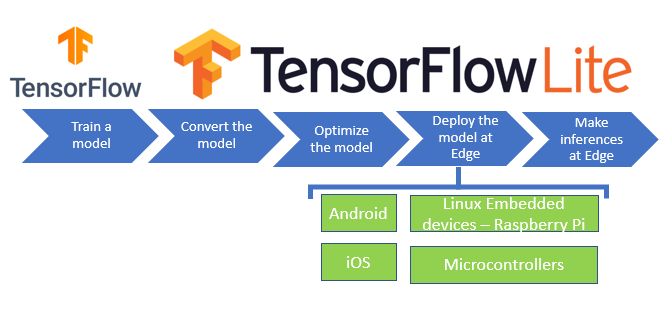
\includegraphics[width=10cm]{images/introduction/training_inference_flow.png}
    \centering
    \caption{From training to edge inference}\label{fig:training_inference}
\end{figure}

The figure \autoref{fig:training_inference} shows a classic life cycle flow of
an intelligent application. A brief explanation of each step:

\begin{itemize}
    \item \textbf{Train a model}: once decided what the task is, the right
        model needs to be used. There are different options: create a custom
        model, use a pre-trained model or use Transfer Learning on a
        pre-trained model.
    \item \textbf{Convert the model}: once the model is trained, it needs to be
        converted in a special format (\texttt{.tflite}) that can be used on
        edge devices in efficient manner.
    \item \textbf{Optimise the model}: that's the key phase where the model is
        optimised to use less space/memory and to have a faster inference by
        decreasing the latency. More details will be presented in section
        \autoref{sec:MO}.
    \item \textbf{Deploy the model at Edge}: once the model has been optimised,
        it is ready to be deployed to the edge device.
    \item \textbf{Make inference at Edge}: this is the last step where finally
        the model is used to do inference on new data that it has never seen
        and hopefully giving expected results in a timely fashion.
\end{itemize}

The above flow shows the big picture of an intelligent application life
cycle~\cite{tflite:intro} and gives an idea of the complexity behind the
creation of an edge intelligent application.
In the rest of the chapter, I will explain what techniques are available in
TensorFlow in order to \textbf{optimise the model}.

\section{Model optimisations for deployment}\label{sec:MO}

To optimise TensorFlow models, the ecosystem offers \textit{TensorFlow Model
Optimisation Toolkit} (abbrev. \textit{TFMOT}) which minimizes the complexity
of optimising machine learning inference.

Inference efficiency is a critical concern when deploying machine learning
models because of latency, memory utilization, and in many cases power
consumption. Particularly on edge devices, such as mobile and Internet of
Things (IoT), resources are further constrained, and model size and efficiency
of computation become a major concern.

Computational demand for training grows with the number of models trained on
different architectures, whereas the computational demand for inference grows
in proportion to the number of users.

Model optimisation is useful, among other things, for:

\begin{itemize}
    \item Reducing latency and cost for inference for both cloud and edge
        devices (e.g.\ mobile, IoT).
    \item Deploying models on edge devices with restrictions on processing,
        memory and/or power-consumption.
    \item Reducing payload size for over-the-air model updates.
    \item Enabling execution on hardware restricted-to or optimised-for
        fixed-point operations.
    \item Optimising models for special purpose hardware accelerators.
\end{itemize}

The available techniques are:

\begin{itemize}
    \item \textbf{Weight Clustering}: Clustered models are those where the
        original model's parameters are replaced with a smaller number of
        unique values.
    \item \textbf{Quantization}: Quantized models are those where we represent
        the models with lower precision, such as 8-bit integers as opposed to
        32-bit float. Lower precision is a requirement to leverage certain
        hardware.
    \item \textbf{Weight Pruning}: Sparse models are those where connections in
        between operators (i.e.\ neural network layers) have been pruned,
        introducing zeros to the parameter tensors.
\end{itemize}

When pre-optimised models and post-training tools do not satisfy your use case,
the next step is to try the different training-time tools.

Training time tools piggyback on the model's loss function over the training
data such that the model can ``adapt'' to the changes brought by the
optimisation technique.~\cite{tfmot:intro}

\subsection{Weight Clustering}
Clustering, or weight sharing, reduces the number of unique weight values in a
model, leading to benefits for deployment. It first groups the weights of each
layer into N clusters, then shares the cluster's centroid value for all the
weights belonging to the cluster.

\begin{figure}[ht]
    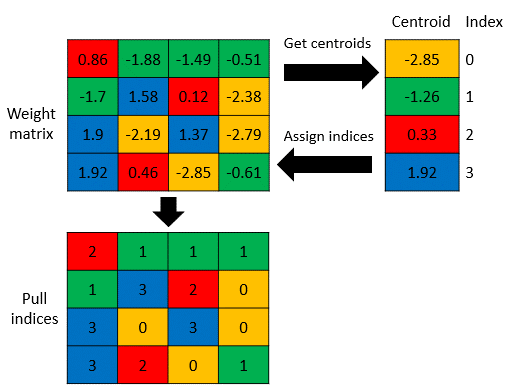
\includegraphics[width=\textwidth]{images/introduction/weight_clustering.png}
    \centering
    \caption{Weight Clustering}\label{fig:weight_clustering}
\end{figure}

A brief explanation of \autoref{fig:weight_clustering}. For example a layer in
the model contains a 4$\times$4 matrix of weights (represented by the
``weight matrix'' in \autoref{fig:weight_clustering}). Each weight is stored
using a float32 value. When the model is saved, 16 unique float32 values are
stored to disk.

Weight clustering reduces the size of the model by replacing similar weights in
a layer with the same value. These values are found by running a clustering
algorithm over the model’s trained weights. The user can specify the number of
clusters (in this case, 4). This step is shown in ``Get centroids'' in the
diagram, and the 4 centroid values are shown in the ``Centroid'' table. Each
centroid value has an index (0\-3).

Next, each weight in the weight matrix is replaced with its centroid’s index.
This step is shown in ``Assign indices''. Now, instead of storing the original
weight matrix, the weight clustering algorithm can store the modified matrix
shown in ``Pull indices'' (containing the index of the centroid values), and
the centroid values themselves.

In this case, the size has been reduced from 16 unique floats, to 4 floats and
16 2-bit indices. The savings increase with larger matrix sizes.

Note that even if we still stored 16 floats, they now have just 4 distinct
values. Common compression tools (like zip) can now take advantage of the
redundancy in the data to achieve higher compression.

Weight clustering has an immediate advantage in reducing model storage and
transfer size across serialization formats, as a model with shared parameters
has a much higher compression rate than one without. This is similar to a
sparse (pruned) model, except that the compression benefit is achieved through
reducing the number of unique weights, while pruning achieves it through
setting weights below a certain threshold to zero. Once a model is clustered,
the benefit of the reduced size is available by passing it through any common
compression tool.

To further unlock the improvements in memory usage and speed at inference time
associated with clustering, specialized run-time or compiler software and
dedicated machine learning hardware is required.~\cite{tfmot:clustering_blog}

This technique brings improvements via model compression. Future framework
support can unlock memory footprint improvements that can make a crucial
difference for deploying deep learning models on embedded systems with limited
resources.

According to Google experiments, models can be compressed up to 5x with minimal
loss of accuracy. Here below results on
vision~\autoref{fig:clustering_image_classification} and speech
models~\autoref{fig:clustering_keyword_spotting}.

\begin{figure}[ht]
    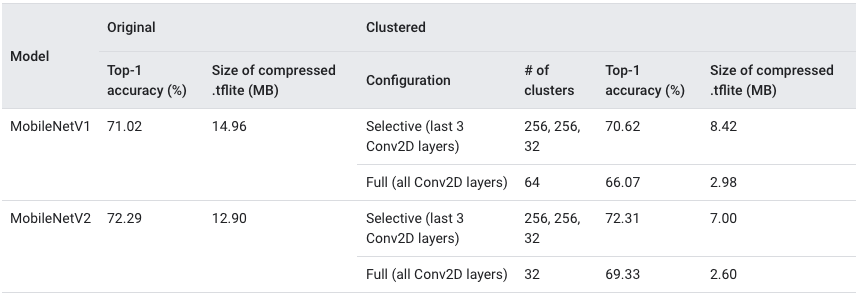
\includegraphics[width=\textwidth]{images/introduction/clustering_image_classification.png}
    \centering
    \caption{Weight Clustering on Image Classification}\label{fig:clustering_image_classification}
\end{figure}


\begin{figure}[ht]
    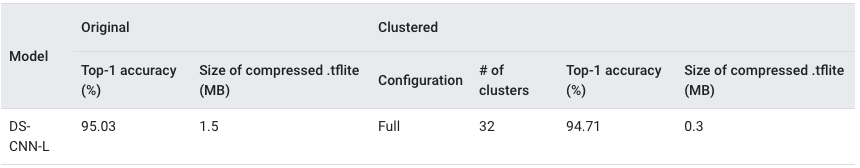
\includegraphics[width=\textwidth]{images/introduction/clustering_keyword_spotting.png}
    \centering
    \caption{Weight Clustering on Keyword Spotting}\label{fig:clustering_keyword_spotting}
\end{figure}

Size of compressed \texttt{.tflite} refers to the size of the zipped
\texttt{.tflite} file obtained from the model from the following process:

\begin{enumerate}
    \item Serialize the Keras model into \texttt{.h5} file
    \item Convert the \texttt{.h5} file into \texttt{.tflite}
    \item Compress the \texttt{.tflite} file into a zip
\end{enumerate}

The weight clustering implementation is based on the \textit{Deep Compression:
Compressing Deep Neural Networks With Pruning, Trained Quantization and Huffman
Coding}~\cite{han2015deep}~\cite{tfmot:clustering}

\subsection{Quantization}
There are two forms of quantization: \textbf{post-training quantization} and
\textbf{quantization aware training (QAT)}. The former is easy to use whilst
the latter often offers better model accuracy.

\subsubsection{Quantization is lossy}
Quantization is the process of transforming an ML model into an equivalent
representation that uses parameters and computations at a lower precision.
This improves the model's execution performance and efficiency

However, the process of going from higher to lower precision is lossy in
nature. As seen in \autoref{fig:quantization}, quantization squeezes a small
range of floating-point values into a fixed number of information buckets.

\begin{figure}[ht]
    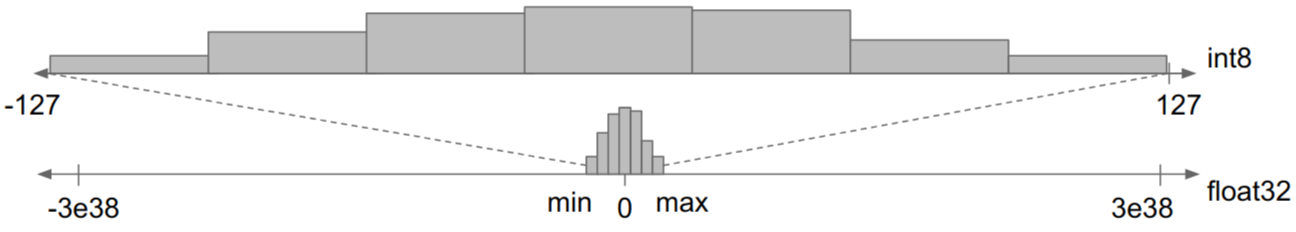
\includegraphics[width=\textwidth]{images/introduction/quantization.png}
    \centering
    \caption{Quantization}\label{fig:quantization}
\end{figure}

This leads to information loss. The parameters (or weights) of a model can now
only take a small set of values and the minute differences between them are
lost. For example, all values in range [2.0, 2.3] may now be represented in one
single bucket. This is similar to rounding errors when fractional values are
represented as integers.

There are also other sources of loss. When these lossy numbers are used in
several multiply-add computations, these losses accumulate. Further, int8
values, which accumulate into int32 integers, need to be rescaled back to int8
values for the next computation, thus introducing more computational
error.~\cite{tfmot:quantization_blog}

\subsubsection{Quantization aware training}
Quantization aware training emulates inference-time quantization, creating a
model that downstream tools will use to produce actually quantized models. The
quantized models use lower-precision (e.g. 8-bit instead of 32-bit float),
leading to benefits during deployment.

Quantization brings improvements via model compression and latency reduction.
With default API, Google has observed that the model shrinks by 4x and 1.5 \-
4x improvements in CPU latency. Eventually, latency improvements can be seen on
compatible machine learning accelerators (e.g.: EdgeTPU and NNAPI).

At the time of writing, QAT is still under development and has some limitations
regarding to its functionality (distributed training, limited support for
Subclassed Models, RNN/LSTM models, stable APIs, etc\ldots)

\begin{figure}[ht]
    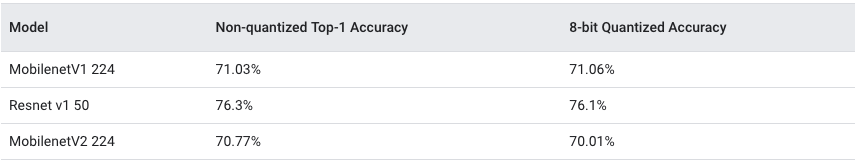
\includegraphics[width=\textwidth]{images/introduction/qat_image_classification.png}
    \centering
    \caption{QAT on Image Classification}\label{fig:qat_image_classification}
\end{figure}

The models in \autoref{fig:qat_image_classification} were tested on Imagenet
and evaluated in both TensorFlow and TFLite.

For background on something similar, see the \textit{Quantization and Training
of Neural Networks for Efficient Integer-Arithmetic-Only Inference}
paper~\cite{Jacob_2018}.
This paper introduces some concepts that this tool uses.
The implementation is not exactly the same, and there are additional concepts
used in this tool (e.g.\ per-axis quantization).~\cite{tfmot:quantization_training}

\subsubsection{Post-training Quantization}
Post-training quantization includes general techniques to reduce CPU and
hardware accelerator latency, processing, power, and model size with little
degradation in model accuracy. These techniques can be performed on an
already-trained float TensorFlow model and applied during TensorFlow Lite
conversion. These techniques are enabled as options in the TensorFlow Lite
converter.

Two types of post-quantization exist:
\begin{itemize}
    \item \textbf{Quantizing weights}: Weights can be converted to types with
        reduced precision, such as 16 bit floats or 8 bit integers. Google
        generally recommends 16-bit floats for GPU acceleration and 8-bit
        integer for CPU execution. At inference, the most critically intensive
        parts are computed with 8 bits instead of floating point.
    \item \textbf{Full integer quantization of weights and activations}:
        Improve latency, processing, and power usage, and get access to
        integer-only hardware accelerators by making sure both weights and
        activations are quantized.  This requires a small representative data
        set. The resulting model will still take float input and output for
        convenience.
\end{itemize}

There are several post-training quantization options to choose from.
\autoref{fig:post_quantization_techniques} shows a summary table of the choices
and the benefits they provide.~\cite{tfmot:quantization_post_training}

\begin{figure}[ht]
    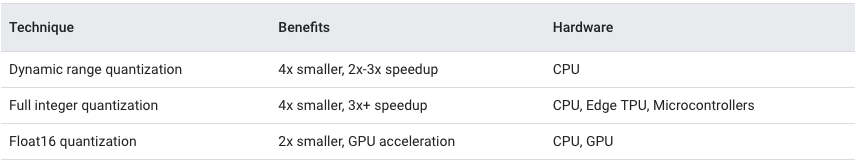
\includegraphics[width=\textwidth]{images/introduction/post_quantization_techniques.png}
    \centering
    \caption{Post-quantization Techniques}\label{fig:post_quantization_techniques}
\end{figure}

Compared to their float counterparts, quantized models are up to 2–4x faster on
CPU and 4x smaller (See \autoref{fig:post_quantization_latency}).

\begin{figure}[ht]
    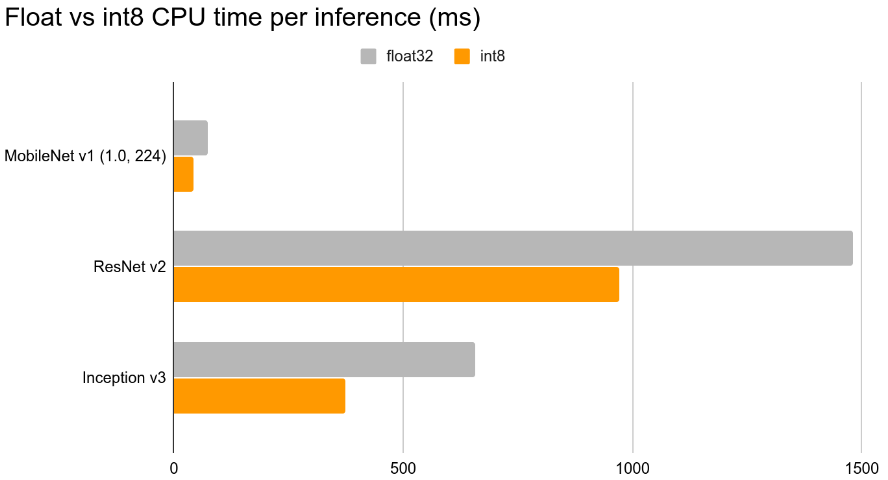
\includegraphics[width=\textwidth]{images/introduction/post_quantization_latency.png}
    \centering
    \caption{Post-quantization latency}\label{fig:post_quantization_latency}
\end{figure}

With just 100 calibration images from ImageNet dataset, fully quantized integer
models have comparable accuracy with their float versions (MobileNet v1 loses
1\%) (See \autoref{fig:post_quantization_accuracy}).

\begin{figure}[ht]
    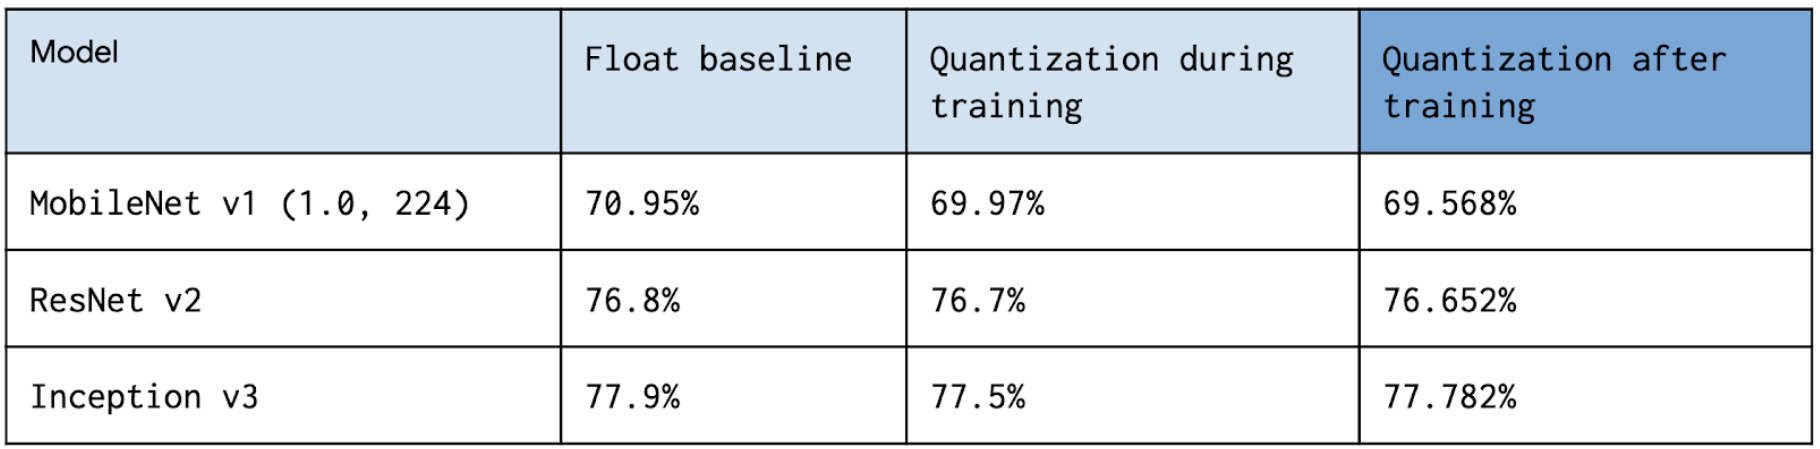
\includegraphics[width=\textwidth]{images/introduction/post_quantization_accuracy.png}
    \centering
    \caption{Post-quantization accuracy}\label{fig:post_quantization_accuracy}
\end{figure}

\subsection{Weight Pruning}
Magnitude-based weight pruning gradually zeroes out model weights during the
training process to achieve model sparsity. Sparse models are easier to
compress, and we can skip the zeroes during inference for latency improvements.

This technique brings improvements via model compression. In the future,
framework support for this technique will provide latency improvements.
Google has seen up to 6x improvements in model compression with minimal loss of
accuracy.

The technique is being evaluated in various speech applications, such as speech
recognition and text-to-speech, and has been experimented on across various
visioni (see \autoref{fig:pruning_image_classification}) and translation
models (see \autoref{fig:pruning_translation}).~\cite{tfmot:pruning}

\begin{figure}[ht]
    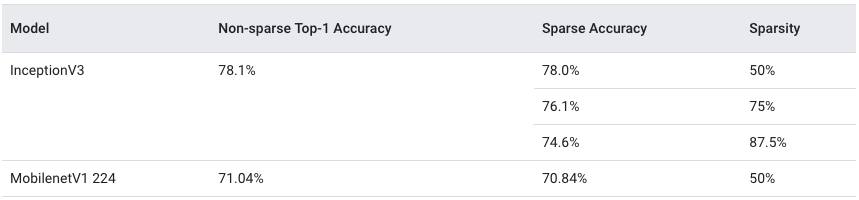
\includegraphics[width=\textwidth]{images/introduction/pruning_image_classification.png}
    \centering
    \caption{Weight Pruning on Image Classification}\label{fig:pruning_image_classification}
\end{figure}

\begin{figure}[ht]
    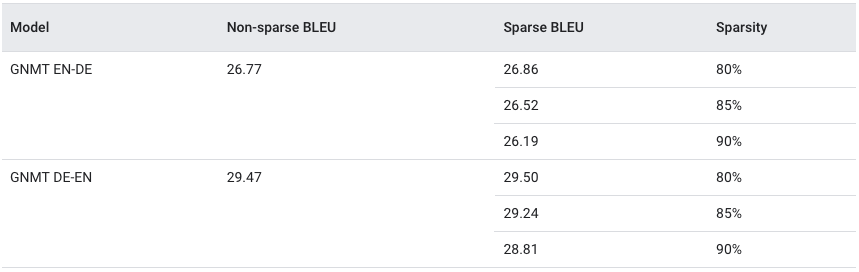
\includegraphics[width=\textwidth]{images/introduction/pruning_translation.png}
    \centering
    \caption{Weight Pruning on Translation}\label{fig:pruning_translation}
\end{figure}

In \autoref{ch:pruning} I will go more in details of this technique.

\subsection{Combine multiple optimisations}
The optimisation techniques shown in \autoref{sec:MO} bring excellent results
in terms of model size and latency.
The model can be optimised further combining those techniques. For instance the
model can be optimised using pruning, post-training quantization and then
compress the result with any compression algorithm (e.g.\ zip, gzip)
Similarly the model can be optimised using clustering, post-training
quantization and compression.
The optimisation can be pushed further including all the previous techniques as
shown in \autoref{fig:collaborative_optimisation}:

\begin{figure}[ht]
    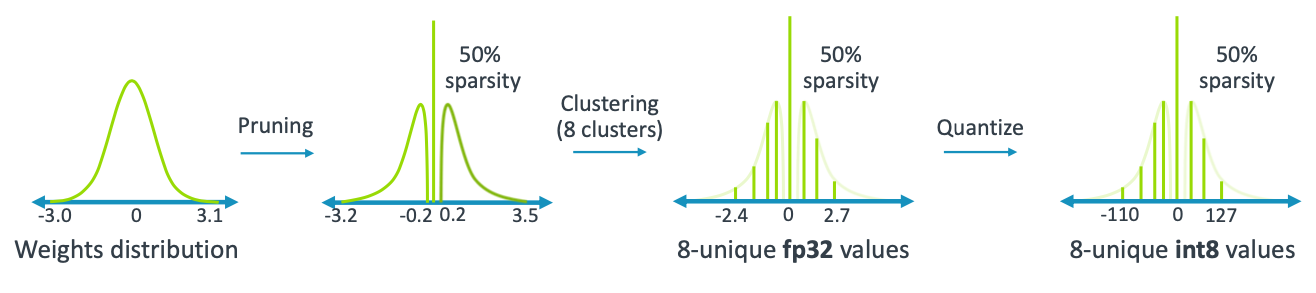
\includegraphics[width=\textwidth]{images/introduction/collaborative_optimisation.png}
    \centering
    \caption{Collaborative optimisation}\label{fig:collaborative_optimisation}
\end{figure}

\begin{enumerate}
    \item \textbf{Weight Pruning}: remove all near-zero weights
    \item \textbf{Weight Clustering}: group all the remaining weights in
        different clusters
    \item \textbf{Quantization}: the weights representing the clusters are
        quantized from floating point at 32 bit to integer at 16/8bit
    \item \textbf{Compression}: the last step is to apply a compression
        algorithm to the model in order to improve deployment
\end{enumerate}

The paper \textit{Deep Compression: Compressing Deep Neural Networks With
Pruning, Trained Quantization and Huffman Coding}~\cite{han2015deep} shows an
optimisation pipeline (See \autoref{fig:combine_multiple_optimisations})

\begin{figure}[ht]
    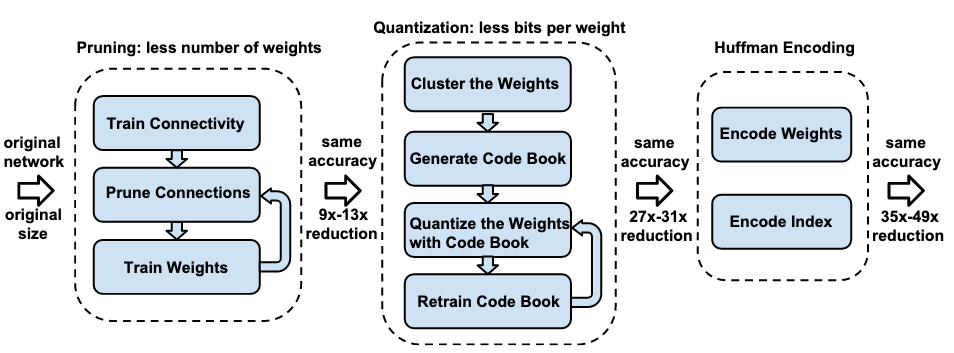
\includegraphics[width=\textwidth]{images/introduction/combine_multiple_optimisations.png}
    \centering
    \caption{Combine multiple optimisations}\label{fig:combine_multiple_optimisations}
\end{figure}

\autoref{fig:combine_multiple_optimisations} shows the three stage compression
pipeline: pruning, quantization (with clustering) and Huffman coding. Pruning
reduces the number of weights by 10×, while quantization/clustering further
improves the compression rate: between 27× and 31×. Huffman coding gives more
compression: between 35× and 49×. The compression rate already included the
meta-data for sparse representation. The compression scheme doesn't incur any
accuracy loss.

    \chapter{Pruning}\label{ch:pruning}
In \autoref{ch:introduction} I gave a brief explanation of few techniques for
doing model optimisation on a neural network. Pruning is one of these and in
the first part of this chapter I give a more detailed explanation.
The second part instead focuses on the core of the thesis: per-layer pruning
configuration with heuristic.

Despite being technical, this chapter is still fairly theoretical and I defer
any code and implementation to \autoref{ch:implementation}.

\section{What's Pruning?}
Neural network pruning is the task of reducing the size of a network by
removing parameters. This compression affects the size of the model, the
latency, the amount of memory and the compute power needed to run the
inference. These metrics need to balanced with the accuracy of the model
itself. I give a more detailed analysis about this trade-off in
\autoref{subsec:tradeoff}

Pruning has been used since the late 1980s but has seen an explosion of
interest in the past decade thanks to the rise of deep neural networks.
It sets its roots with a couple of classic papers:\textit{Optimal Brain
Damage}~\cite{lecun-90b} and \textit{Optimal Brain Surgeon}\cite{hassibi-93}

In the last decade (2010\-2020) a few dozens of papers have been published in
literature about pruning and all of them have been showing that pruning is an
effective technique that can be applied to a variety of neural network on
different fields (image and speech recognition, text processing, etc\ldots).
Moreover they highlights that pruning is a versatile technique as, I said
earlier, it has a positive impact on multiple metrics, all important for a
better edge deployment of the model.

How does pruning reduce the size of a model? The basic principle is to prune
(remove) unnecessary neurones or weights (see \autoref{fig:pruning_weights_neurons}):

\begin{figure}[ht]
    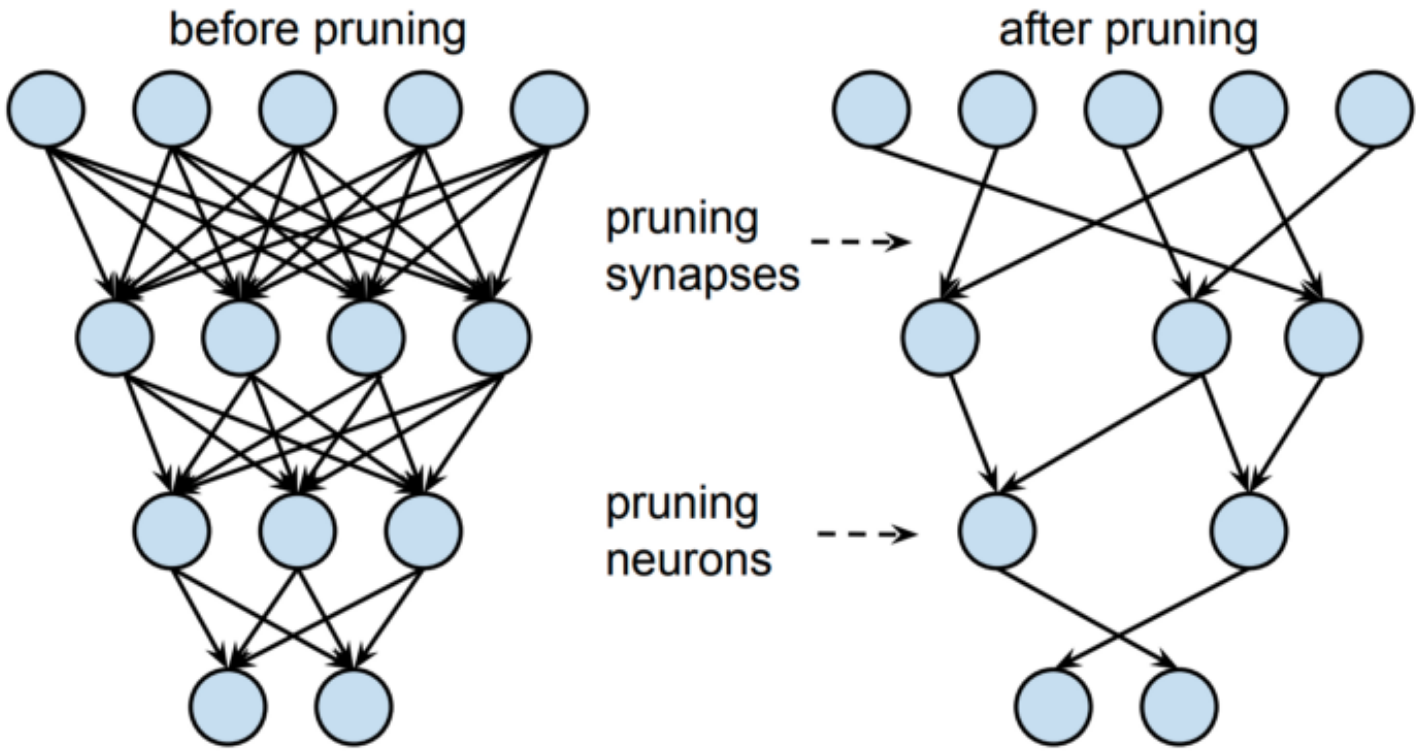
\includegraphics[width=8cm]{images/pruning/pruning_weights_neurons.png}
    \centering
    \caption{Pruning weights and neurons}\label{fig:pruning_weights_neurons}
\end{figure}

\begin{itemize}
    \item \textbf{weights}: this is done by setting individual parameters to
        zero and making the network sparse. The effect will be to maintain the
        same architecture of the network but lowering down the number of
        parameters.
    \item \textbf{neurons}: this is done by removing the entire node from the
        network with all its connections. This would make the network
        architecture smaller but with the target to keep the accuracy of the
        starting network.
\end{itemize}

\subsection{Pruning techniques}
The main problem in pruning is to understand what to prune. Of course the goal
is to remove nodes and/or weights that are less useful. There are different
methods to understand what to prune with very little or no effect on accuracy.
Below e brief description of different techniques.

\subsubsection{Magnitude Pruning}
Functions can be a very simple case of a neural network. Its coefficients can
be changed in order to learn the input data points. There are coefficients
that, despite changing their values, they won't change the behaviour of the
function and these are referred as \textbf{non-significant}.
In neural networks these coefficients are weights and biases: they are
\textbf{trainable parameters} and the same non-significant concept can be
applied to them with bit more complexity.

During the back-propagation (gradient descent) some weights are updated with
larger gradient magnitudes (both positive and negative) than the others.
These weights are the \textbf{significant} ones and the weights receiving very
small gradients can be considered as \textbf{non-significant} as their impact
is minimal to the optimization of the loss function.
After the training, the weight magnitude of every layer can be explored and
check which weights are significant.

So the weight magnitude is the criteria for pruning the neural network.
At this point a \textbf{threshold} is specified and all the weights below this
threshold are considered non-significant. This is usually combined with a
\textbf{sparsity target} the network should achieve.
The \textbf{non-significant weights will be zeroed}, cancelling effectively
their impact in the neural network.
This can be applied to biases as well (to any trainable parameter to be
precise).

Once the pruning is done it's always advisable to retrain the network in order
to compensate for any drop in performance. It's worth noticing that during the
retraining the pruned weights won't be updated.~\cite{magnitude_pruning}

Magnitude pruning is the technique I will be using in
\autoref{ch:implementation}.

\subsubsection{Channel Pruning}
Channel pruning is a technique specifically for CNN (Convolutional Neural
Network) as it rely on the architecture of this type of networks. The building
blocks of a CNN are (see \autoref{fig:cnn}):

\begin{figure}[ht]
    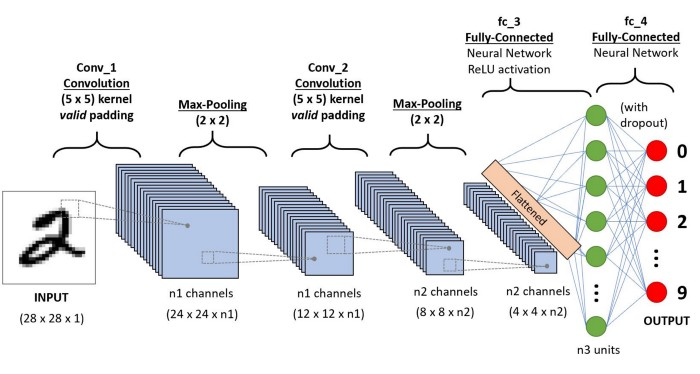
\includegraphics[width=\textwidth]{images/pruning/cnn.jpeg}
    \centering
    \caption{Convolutional Neural Network Architecture}\label{fig:cnn}
\end{figure}

\begin{itemize}
    \item \textbf{Convolutional layer}: it is the core building block of a CNN\@.
        A convolution is the simple application of a filter to an input that
        results in an activation. Repeated application of the same filter to an
        input results in a map of activations called a feature map, indicating
        the locations and strength of a detected feature in an input, such as
        an image.
    \item \textbf{Pooling layer}: it provide an approach to down sampling
        feature maps by summarizing the presence of features in patches of the
        feature map. Two common pooling methods are average pooling and max
        pooling that summarize the average presence of a feature and the most
        activated presence of a feature respectively.
    \item \textbf{ReLU layer}: ReLU stands for \textbf{Rectified Linear Unit}
        and it is a piecewise linear function that will output the input
        directly if it is positive, otherwise, it will output zero. It has
        become the default activation function for many types of neural
        networks because a model that uses it is easier to train and often
        achieves better performance (see \autoref{fig:relu})
\begin{figure}[ht]
    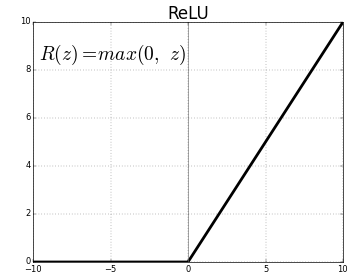
\includegraphics[width=8cm]{images/pruning/relu.png}
    \centering
    \caption{Rectified Linear Unit activation function}\label{fig:relu}
\end{figure}
    \item \textbf{Fully connected layer}: after several convolutional and max
        pooling layers, the high-level reasoning in the neural network is done
        via fully connected layers. Neurons in a fully connected layer have
        connections to all activations in the previous layer, as seen in
        non-convolutional artificial neural networks.
    \item \textbf{Loss layer}: it specifies how training penalizes the
        deviation between the predicted (output) and true labels and is
        normally the final layer of a neural network. Various loss functions
        appropriate for different tasks may be used. Softmax loss is used for
        predicting a single class of K mutually exclusive classes.
        Sigmoid cross-entropy loss is used for predicting K independent
        probability values in [0, 1]. Euclidean loss is used for regressing to
        real-valued labels.\cite{cnn}
\end{itemize}

\autoref{fig:channel_pruning} shows the channel pruning algorithm for a
single convolutional layer.
The aim is to reduce the number of channels of feature map B, while maintaining
outputs in feature map C.
Once the channels are pruned, corresponding channels of the filters that take
these channels as input can be removed. Moreover, filters that produce these
channels can be removed as well. It is clear that channel pruning involves
two key steps.

\begin{figure}[ht]
    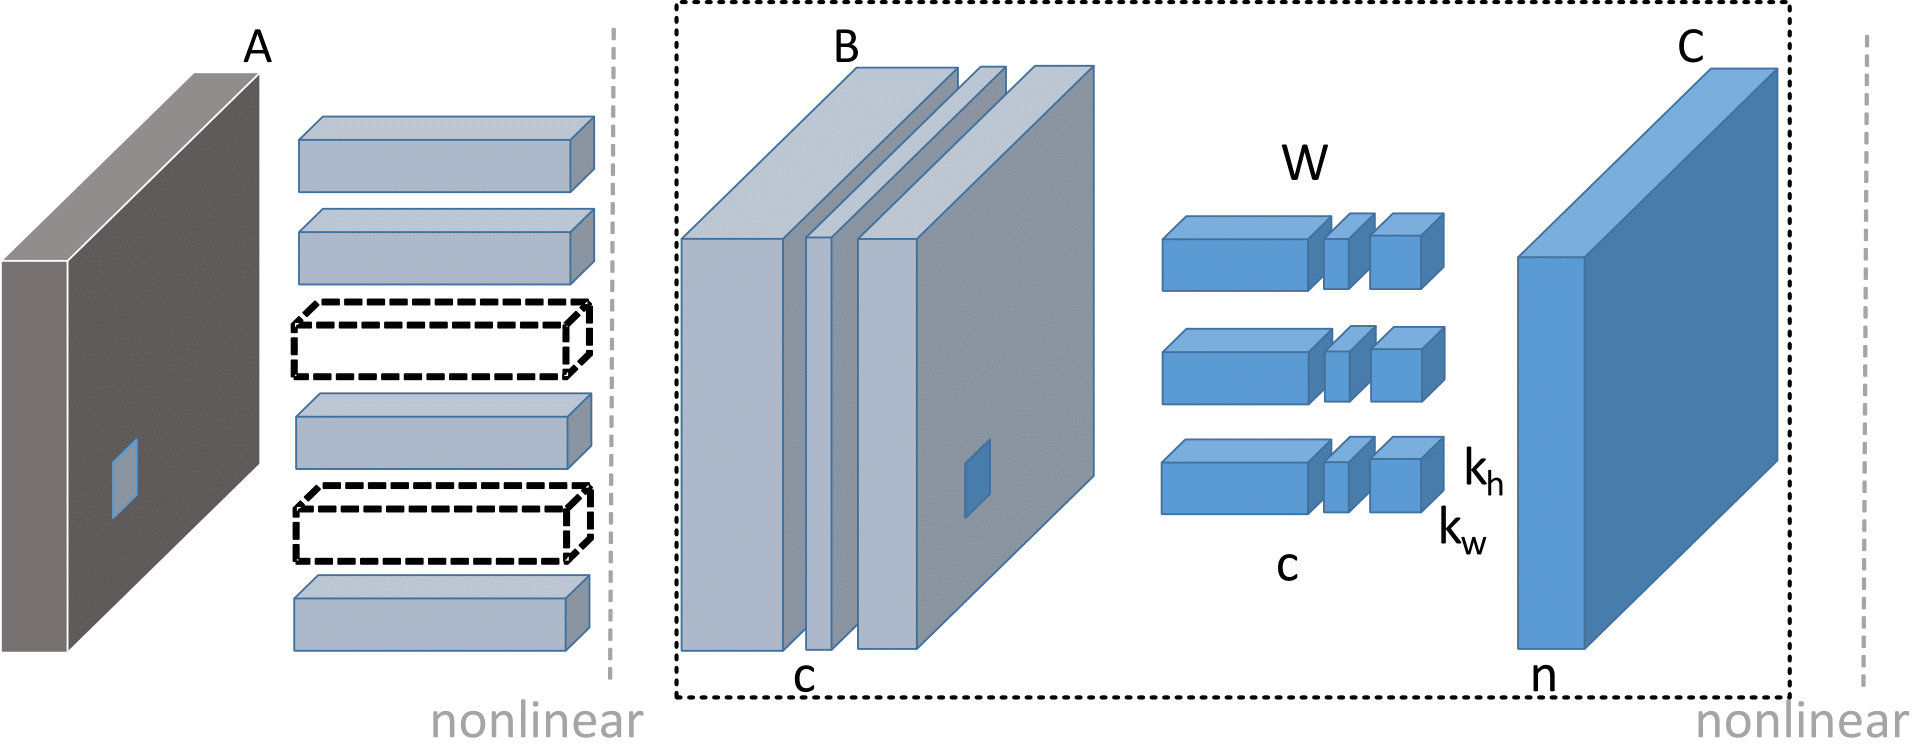
\includegraphics[width=8cm]{images/pruning/channel_pruning.png}
    \centering
    \caption{Channel Pruning for accelerating a CNN}\label{fig:channel_pruning}
\end{figure}

The first is the channel selection, since a proper channel combination to
maintain as much information needs to be selected.
The second is reconstruction. The following feature maps need to be
reconstructed using the selected channels. Motivated by this, the process is an
iterative two-step algorithm.

In the first step, the aim is to select most representative channels.
Since an exhaustive search is infeasible even for tiny networks, a LASSO
regression based method needs to be performed to figure out representative
channels and prune redundant ones.

In the second step, outputs are reconstructed with remaining channels with
linear least squares.

The whole model can be pruned applying the approach layer by layer
sequentially. For each layer, input volumes are obtained from the current input
feature map, and output volumes from the output feature map of the un-pruned
model.\cite{He_2017}

\subsubsection{Structured Pruning}
\lipsum[1]

\subsection{Pruning pipeline}
Training, pruning, fine-tuning
1506.02626 \- Learning both Weights and Connections for Efficient Neural Networks
\lipsum[1]

\subsection{Practical examples with Pruning}
\lipsum[1]

\subsection{Sparsity-accuracy trade-offs}\label{subsec:tradeoff}
\lipsum[1]

\section{Per-Layer Pruning Configuration With Heuristic}\label{sec:heuristic}
\lipsum[1]

\subsection{What's a heuristic?}
\lipsum[1]

\subsection{Heuristic details}
Explain in details the technique and the reasons behind
\lipsum[1]

\subsection{Custom heuristic formula}
\lipsum[1]

    \chapter{Implementation}\label{ch:implementation}
This chapter shows the code that implements the pruning with heuristic
explained in \autoref{sec:heuristic}.

\section{Codebase}
The whole implementation is contained in the TensorFlow Model Optimization
(TFMOT)
repository\footnote{\url{https://github.com/tensorflow/model-optimization}}
This because the pruning with heuristic is a training-time optimization and it
is an improvements of the current pruning API\@.

At the time of writing the code is not public yet: the upstream process usually
lasts for months and it involves various discussion with Google.

In the next subsections I show briefly the current API for pruning, the API for
pruning with heuristic and then some explanation of the code behind the
implementation.

\subsection{Pruning API in TFMOT}
Pruning API in TFMOT are very easy to use. Below an example that shows how to
prune a model. I skip the details of building the model and focus more on the
pruning. In \autoref{sec:workingexamples} I'll show details on how to create a
model.

\begin{lstlisting}[language=Python, label={lst:tfmotpruningexample},
    caption=Pruning example in TFMOT]
import tempfile
import os

import tensorflow as tf
import numpy as np

from tensorflow import keras
import tensorflow_model_optimization as tfmot

# Load MNIST dataset
mnist = keras.datasets.mnist
(train_images, train_labels), (test_images, test_labels) = mnist.load_data()

# Normalize the input image so that each pixel value is between 0 to 1.
train_images = train_images / 255.0
test_images = test_images / 255.0

# Build and train the model
model = build_and_train_your_model()

prune_low_magnitude = tfmot.sparsity.keras.prune_low_magnitude

# Compute end step to finish pruning after 2 epochs
batch_size = 128
epochs = 2

# 10% of training set will be used for validation set
validation_split = 0.1

num_images = train_images.shape[0] * (1 - validation_split)
end_step = np.ceil(num_images / batch_size).astype(np.int32) * epochs

# Define pruning parameters
pruning_params = {
  "pruning_schedule": tfmot.sparsity.keras.PolynomialDecay(
    initial_sparsity=0.4,
    final_sparsity=0.8,
    begin_step=0,
    end_step=end_step)
}

model_for_pruning = prune_low_magnitude(model, **pruning_params)

# "prune_low_magnitude" requires a recompile
model_for_pruning.compile(
  optimizer='adam',
  loss=tf.keras.losses.SparseCategoricalCrossentropy(from_logits=True),
  metrics=['accuracy']
)

logdir = tempfile.mkdtemp()

callbacks = [
  tfmot.sparsity.keras.UpdatePruningStep(),
  tfmot.sparsity.keras.PruningSummaries(log_dir=logdir),
]

# Fine tune with pruning for two epochs
model_for_pruning.fit(
  train_images,
  train_labels,
  batch_size=batch_size,
  epochs=epochs,
  validation_split=validation_split,
  callbacks=callbacks
)

# Evaluate the accuracy of the pruned model
_, model_for_pruning_accuracy = model_for_pruning.evaluate(
  test_images,
  test_labels,
  verbose=0
)
print('Pruned test accuracy:', model_for_pruning_accuracy)
\end{lstlisting}

The \autoref{lst:tfmotpruningexample} can be split in the following three
sections:

\begin{enumerate}
    \item Define and train the model (lines 1--31)
    \item Setup the model pruning (lines 33--49)
    \item Prune, fine tuning weights and evaluate the model (lines 51--74)
\end{enumerate}

Below more details of the three sections.

\subsubsection{Define and train the model}
Apart the usual imports at the top of the file, the
MNIST\footnote{\url{http://yann.lecun.com/exdb/mnist/}} dataset is loaded
generating the split between training and test images (line 12).
10\% of the dataset is kept for validation purposes (line 28)

\texttt{build\_and\_train\_your\_model} is a custom function to define and
train the model.

\texttt{batch\_size = 128} defines the number of samples that will be
propagated through the network. In this case 128 samples at the time are taken
and propagated through the network.
The main advantage is the memory usage: the memory footprint is the equivalent
of loading 128 samples of the training data at any time.

\texttt{epochs = 2} means that the training will do a full pass twice over the
full training set. Please note that in this case the epochs defines how many
passes the pruning training will do.

Finally the number if images are the full set minus 10\% reserved to
validation (line 30). The shape of \texttt{train\_images} is the following

\begin{lstlisting}[language=Python, caption=Shape of train\_images]
>>> train_images.shape
(60000, 28, 28)
\end{lstlisting}

The first element is the number if images present in the dataset.

With all data above, the \texttt{end\_step} is then calculated.

\subsubsection{Setup the model pruning}
In this block, the model is prepared for the pruning activity.
This is done by defining the pruning parameters. In this case only the pruning
schedule has been defined (lines 34--40).

\texttt{prune\_low\_magnitude} accepts as parameters the trained model and the
dictionary with the pruning settings: the function has the goal to augment the
model layers with pruning information taken by the pruning parameters.
The resulting model then is compiled again (lines 45--49) before calling the
\texttt{fit} method.

\subsubsection{Prune, fine tuning weights and evaluate the model}
After the compilation of the model, it is finally time to prune the model.

The \texttt{UpdatePruningStep} callback is the one that updates pruning
wrappers with the optimizer step. Not adding this callback to the \texttt{fit}
method will result in throwing an error.

Finally the \texttt{fit} method fine-tunes the weights thanks to the callbacks
definition above.
After the pruning, the model is evaluated and return the accuracy of the new
model (lines 69--74)

\subsection{Pruning API with Heuristic}
If the heuristic based pruning needs to be applied, few lines of the above
example need to be changed.

\begin{lstlisting}[language=Python, caption=Pruning with Heuristic]
|*\ldots*|

from tensorflow_model_optimization.python.core.api.experimental import (
    sparsity_distribution,
)

|*\ldots*|

pruning_params = {
  "pruning_schedule":
    tfmot.sparsity.keras.PolynomialDecay(
      initial_sparsity=0.4,
      final_sparsity=0.8,
      begin_step=0,
      end_step=end_step
    ),
  "sparsity_distribution":
    sparsity_distribution.HeuristicSparsityDistribution(),
}

|*\ldots*|

model_for_pruning = \
  sparsity_distribution.prune_low_magnitude_custom_distribution(
    sequential_model, **pruning_params
  )

|*\ldots*|
\end{lstlisting}

The main changes compared to classical API are:

\begin{itemize}
    \item Import the new experimental module (lines 3--5)
    \item Define the heuristic based sparsity distribution in the pruning
        parameters (lines 17--18)
    \item \texttt{prune\_low\_magnitude\_custom\_distribution} is called in
        favour of the classic method (\texttt{prune\_low\_magnitude})
\end{itemize}

There are few key points to highlight in the implementation:

\begin{itemize}
    \item \texttt{HeuristicSparsityDistribution} is a subclass of \linebreak
        \texttt{SparsityDistribution}: the subclass needs to implement
        \linebreak
        \texttt{sparsity\_function\string(self, model, target\_pruning\_ratio\string)}
        method in order to define the custom distribution to apply to model's
        layers.

        Actual layer's information are stored in a data structure inside the
        instance of the class and it will be exported using
        \texttt{get\_sparsity\_map} method.

        The class has also a mechanism that checks if the projected sparsity
        distribution honours the target pruning ration set by the user: in case
        it doesn't, it prints a warning message.
    \item \texttt{prune\_low\_magnitude\_custom\_distribution} is a wrapper
        around the classic \texttt{prune\_low\_magnitude} function. It has a
        similar signature and takes an additional parameter:
        \texttt{sparsity\_distribution} which should be an instance of
        \texttt{SparsityDistribution}.

        The \texttt{sparsity\_distribution} create the \texttt{sparsity\_map}
        which will be used to wrap model's layer with sparsity distribution
        information.

        The function will revert back to the classic
        \texttt{prune\_low\_magnitude} in the following cases:
        \texttt{sparsity\_distribution} is not an instance of \linebreak
        \texttt{SparsityDistribution} or it is not defined and the object to
        prune is not a sequential of functional model. In this cases a warning
        will be printed saying the heuristic cannot be applied.
\end{itemize}

For a deeper understanding of the implementation,
\autoref{appendix:distribution.py} shows the code of
\texttt{HeuristicSparsityDistribution} and \texttt{SparsityDistribution},
whilst \autoref{appendix:prune.py} shows
\texttt{prune\_low\_magnitude\_custom\_distribution}

\section{Fully working examples}\label{sec:workingexamples}
\lipsum[1]

\subsection{MNIST}
\lipsum[1]

\subsection{DS-CNN-L}
\lipsum[1]

    \chapter{Results}\label{ch:results}
In this chapter I show how the pruning with heuristic affects MobileNet
v1\cite{howard2017mobilenets} based models. The experiments will be run using
both CIFAR-10\cite{cifar_10} and ImageNet 2012\cite{imagenet_cvpr09}.
Before showing to the results, I'll give an overview about MobileNet v1
architecture and the respective datasets used in the experiments.

\section{MobileNet v1}
MobileNet is a class of efficient models for mobile and embedded vision
applications (\autoref{fig:mobilenet_applications}) developed by Google.
It is based on a streamlined architecture that uses depthwise separable
convolutions to build light weight deep neural networks.

\begin{figure}[ht]
    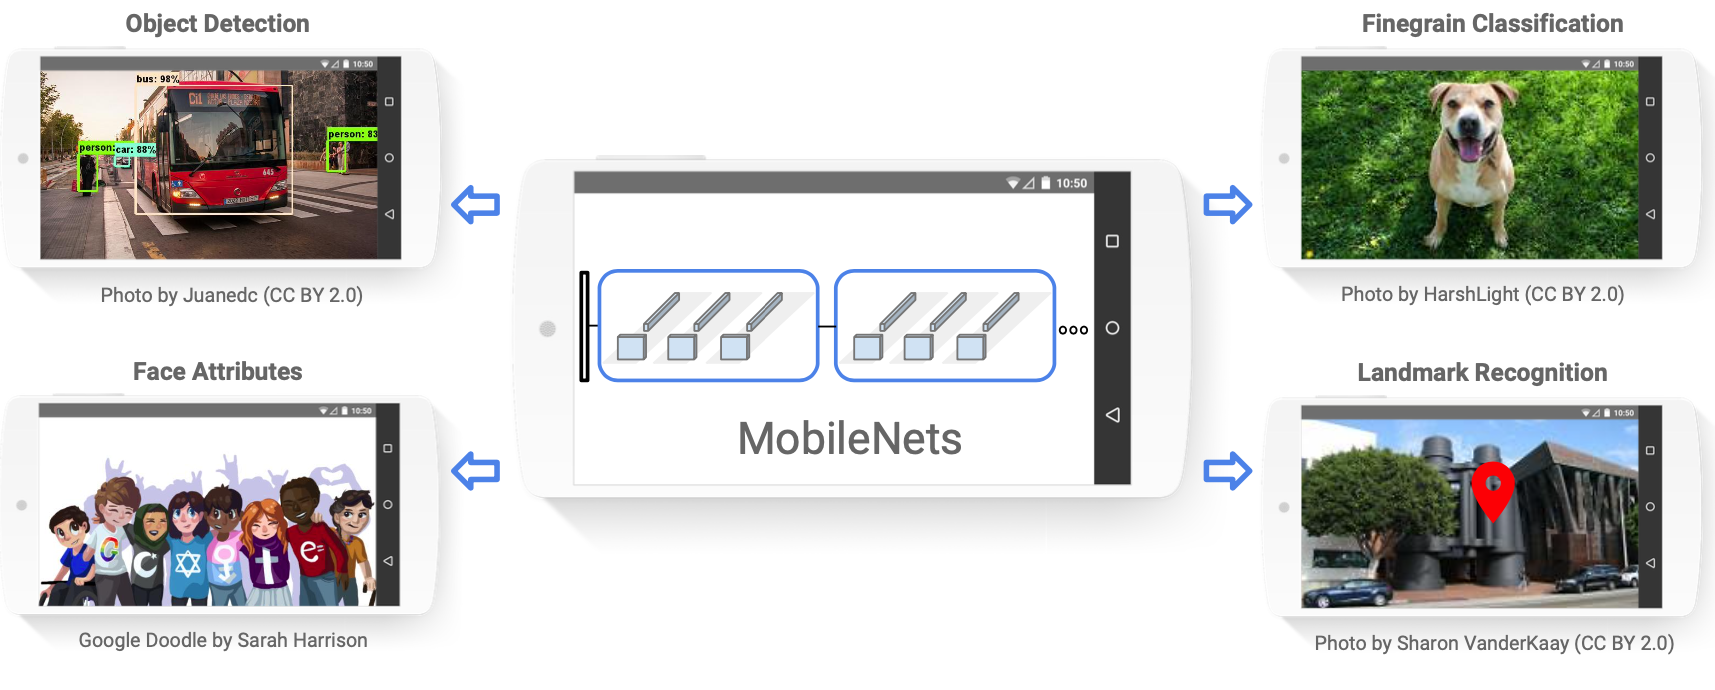
\includegraphics[width=\textwidth]{images/results/mobilenet_applications.png}
    \centering
    \caption{MobileNet applications}\label{fig:mobilenet_applications}
\end{figure}

Convolutional neural networks have been more popular in the recent years and
their accuracy increased thanks to more complex architecture increasing their
size whilst impacting negatively in speed. In many real world applications,
these networks need to run on edge devices with limited resources and the
inferences need to be carried out in a timely fashion.

The main focus of MobileNet is to increase the efficiency of the network by
decreasing the number of parameters by not compromising
performance\cite{review_mobilenet}.

\subsection{Depthwise Separable Convolution}
Depthwise separable convolution is the core basis of MobileNet architecture. It
is a \textbf{depthwise convolution followed by a pointwise convolution}.

A normal convolution is shown in \autoref{fig:convolution}

\begin{figure}[ht]
    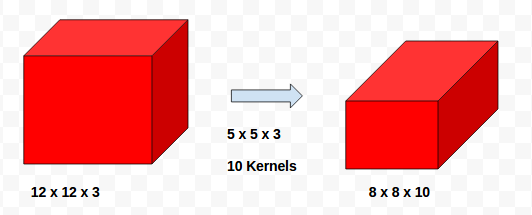
\includegraphics[width=10cm]{images/results/convolution.png}
    \centering
    \caption{Convolution}\label{fig:convolution}
\end{figure}

In the figure there is an input image size of $12\times12\times3$ and the
kernel (or filter) is $5\times5\times3$ with stride = 1. There are though 10
kernels to apply and this gives an output image of $8\times8\times10$.
The total computational cost is \bm{$12\times12\times5\times5\times3\times10 =
108000$}.

There are the following dimensions:
\begin{itemize}
    \item Input image: \bm{$D_f \times D_f \times M$}
    \item Output image: \bm{$D_f \times D_f \times N$}
    \item Convolution kernel: \bm{$D_k \times D_k \times M \times N$}
\end{itemize}

So in a normal convolution the total computational cost is
\bm{$D_k \times D_k \times M \times N \times D_f \times D_f$}

The above convolution can be divided  in 2 phases:
\begin{enumerate}
    \item Depthwise convolution
    \item Pointwise convolution
\end{enumerate}

The first one is the \textbf{depthwise convolution} and it is shown in
\autoref{fig:depthwise_convolution}.

\begin{figure}[ht]
    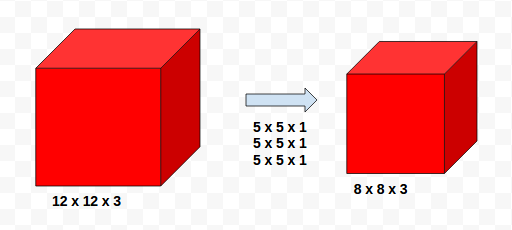
\includegraphics[width=10cm]{images/results/depthwise_convolution.png}
    \centering
    \caption{Depthwise convolution}\label{fig:depthwise_convolution}
\end{figure}

In this case the input has 3 channels and there are 3 $5\times5\times1$
kernels. These 3 kernels are applied to the three channels respectively
producing 3 $8\times8\times1$ output. When the 3 outputs are stacked the final
output is $8\times8\times3$.

The second phase is the \textbf{pointwise convolution} as shown in
\autoref{fig:pointwise_convolution}.

\begin{figure}[ht]
    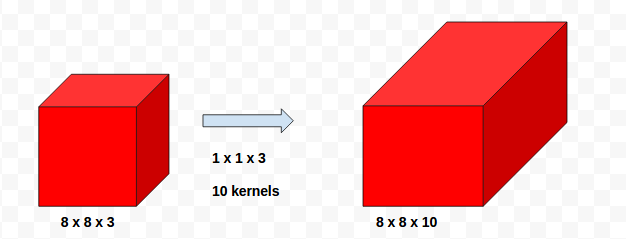
\includegraphics[width=10cm]{images/results/pointwise_convolution.png}
    \centering
    \caption{Pointwise convolution}\label{fig:pointwise_convolution}
\end{figure}

The output image of the previous step is the input image for this step.
The convolution is done using a $1\times1\times3$ kernel on the input image
producing a feature map. Repeating this using 10 different $1\times1\times3$
kernels will produce 10 different feature maps that will be stacked together.

The computation for each step is:
\begin{enumerate}
    \item Depthwise convolution: \bm{$12 \times 12 \times 5 \times 5 \times 3 =
        10800$}
    \item Pointwise convolution: \bm{$8 \times 8 \times 3 \times 10 = 1920$}
\end{enumerate}

Therefore the total number of computations is \textbf{10800 + 1920 = 12720}

More generically the computational cost is \bm{$D_k \times D_k \times M \times
D_f \times D_f + M \times N \times D_f \times D_f$}

In this specific case using a kernel of $3 \times 3$ there is about 8 to 9
times less computational reduction: \bm{$108000 / 12720 \approx 8.45$}

\subsection{MobileNet architecture}
The network architecture is built on depthwise separable convolutions except
for the first layer which is a full convolution

There are 28 convolutional layers (counting depthwise and pointwise layers) and
1 fully connected layer followed by a softmax layer
(\autoref{fig:mobilenet_architecture}).

\begin{figure}[ht]
    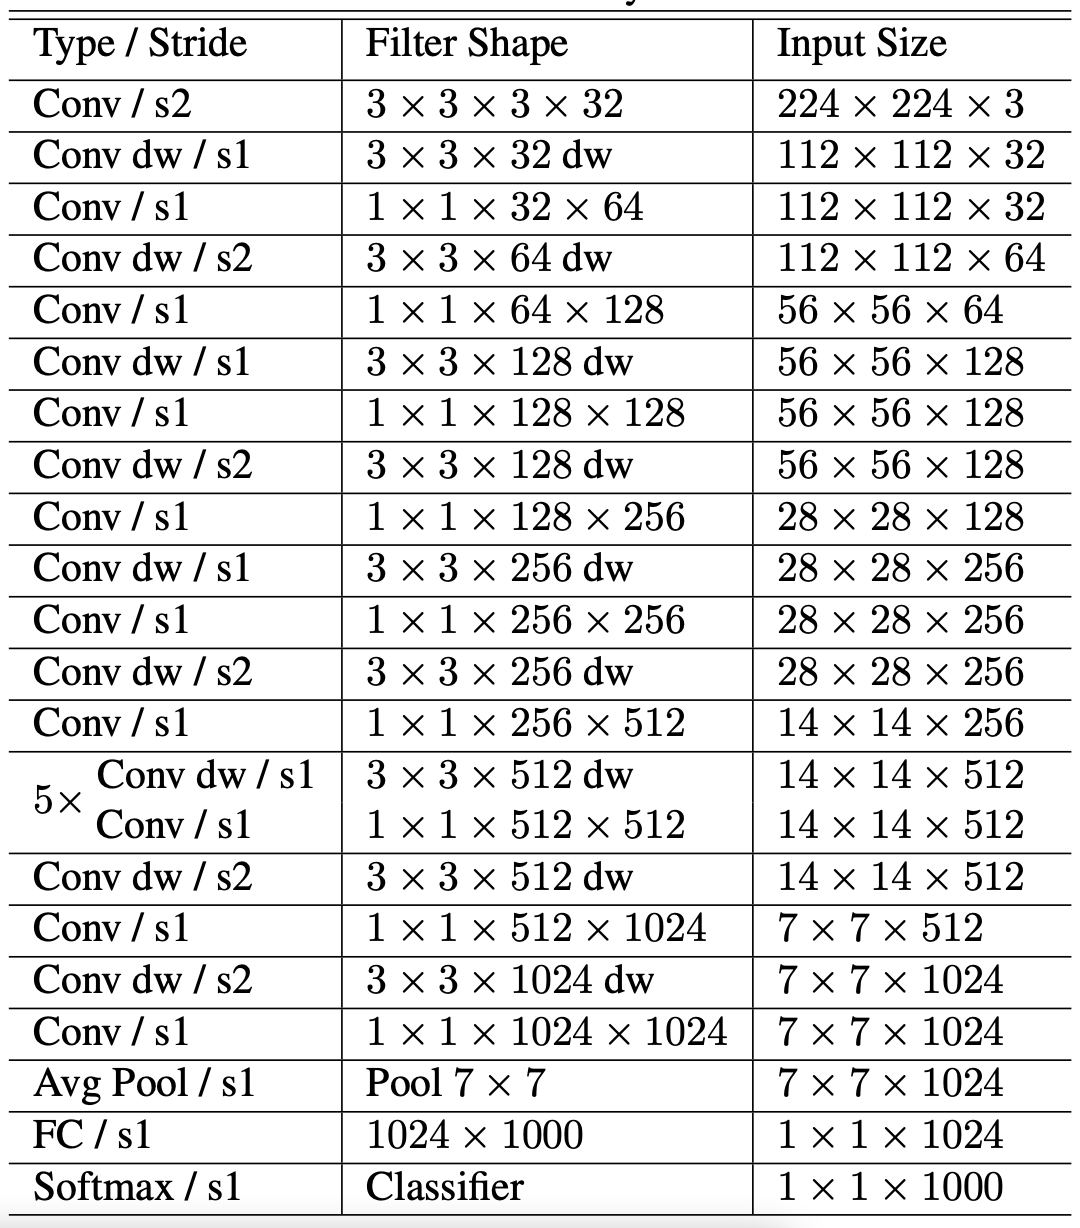
\includegraphics[width=10cm]{images/results/mobilenet_architecture.png}
    \centering
    \caption{MobileNet architecture}\label{fig:mobilenet_architecture}
\end{figure}

All layers are followed by a batch normalization and ReLU non linearity
(\autoref{fig:mobilenet_convolution}) with the exception of the final fully
connected layer which has no non linearity and feeds into a softmax layer for
classification.
As seen earlier in the thesis, the softmax is used to to predict a single class
of K mutually exclusive classes. In the case of MobileNet, when used with
ImageNet, it can classify up to 1000 classes.

\begin{figure}[ht]
    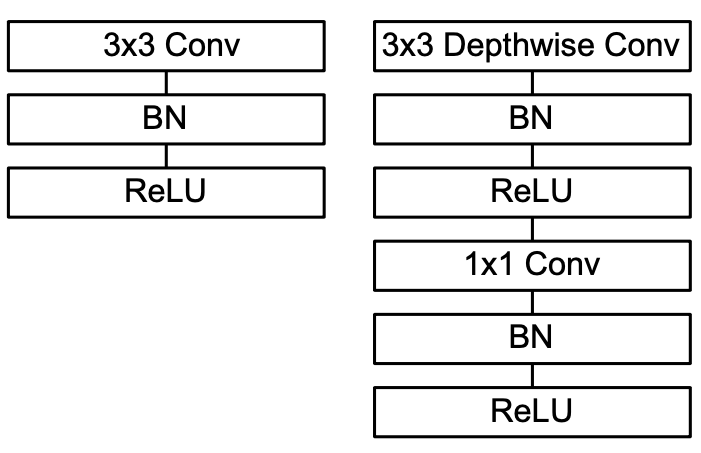
\includegraphics[width=8cm]{images/results/mobilenet_convolution.png}
    \centering
    \caption{Normal convolution vs MobileNet convolution}\label{fig:mobilenet_convolution}
\end{figure}

\subsection{Width Multiplier}
MobileNet has been developed to be small and low latency but sometimes specific
use cases or applications need the model to be faster and smaller.
In order to construct these smaller and less computationally expensive models
a very simple parameter \bm{$\alpha$} called width multiplier has been
introduced.

The role of the width multiplier $\alpha$ is to thin a network uniformly at
each layer: the number of input channels M becomes $\alpha M$ and the number of
output channels N becomes $\alpha N$.

So depth wise separable computational cost becomes \bm{$D_k \times D_k \times
\alpha M \times D_f \times D_f + \alpha M \times \alpha N \times D_f \times
D_f$} where $\alpha \in \interval[open left]{0}{1}$ with typical settings of 1,
0.75, 0.5, 0.25.

The \autoref{fig:mobilenet_widthmultiplier} shows the impact that $\alpha$ has
on accuracy, numbers of operations and parameters.

\begin{figure}[ht]
    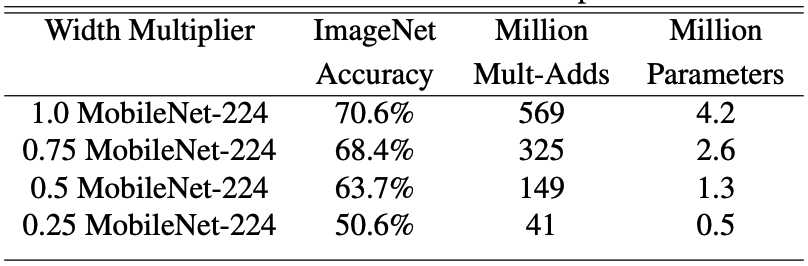
\includegraphics[width=10cm]{images/results/mobilenet_widthmultiplier.png}
    \centering
    \caption{Width multiplier impact}\label{fig:mobilenet_widthmultiplier}
\end{figure}

In this thesis I consider \bm{$\alpha = 1$} to be the baseline.

\subsection{Resolution Multiplier}
The second hyper-parameter to reduce the computational cost of a neural network
is a resolution multiplier \bm{$\rho$}. This can be applied to the input image
and the internal representation of every layer is subsequently reduced by the
same multiplier.
Including $\rho$, the computational cost becomes \bm{$D_k \times D_k \times
\alpha M \times \rho D_f \times \rho D_f + \alpha M \times \alpha N \times \rho
D_f \times \rho D_f$} where $\rho \in \interval[open left]{0}{1}$i which is
typically set implicitly so that the input resolution of the network is 224,
192, 160 or 128.

The \autoref{fig:mobilenet_resolutionmultiplier} shows the impact that $\rho$
has on accuracy, numbers of operations and parameters.

\begin{figure}[ht]
    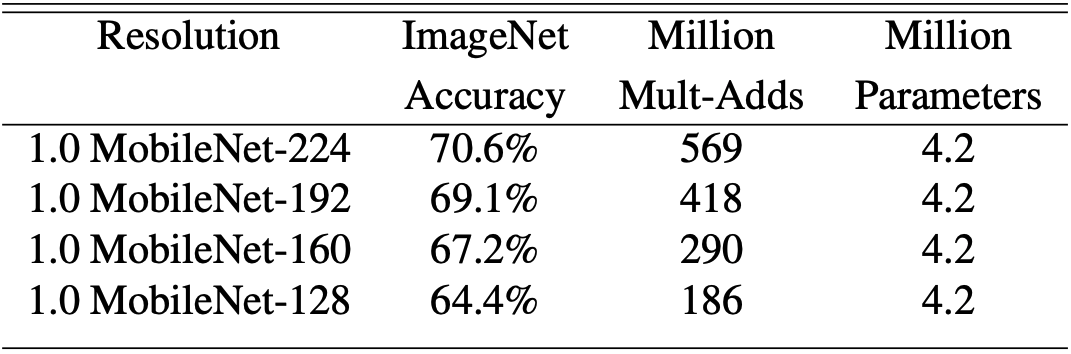
\includegraphics[width=10cm]{images/results/mobilenet_resolutionmultiplier.png}
    \centering
    \caption{Resolution multiplier impact}\label{fig:mobilenet_resolutionmultiplier}
\end{figure}

In this thesis I consider \bm{$\rho = 1$} to be the baseline.

\section{Datasets: CIFAR-10 and ImageNet}
In this section, I give a brief explanation of CIFAR-10 and ImageNet datasets.

\subsection{CIFAR-10 dataset}
The CIFAR-10 dataset (Canadian Institute For Advanced Research) is a collection
of images that are commonly used to train neural networks. It is one of the
most widely used datasets for machine learning research.

It consists of \textbf{60000} \bm{$32 \times 32$} colour images in
\textbf{10 classes}, with 6000 images per class. There are 50000 training
images and 10000 test images.

The dataset is divided into five training batches and one test batch, each with
10000 images. The test batch contains exactly 1000 randomly-selected images
from each class. The training batches contain the remaining images in random
order, but some training batches may contain more images from one class than
another. Between them, the training batches contain exactly 5000 images from
each class.

The 10 different classes represent airplanes, cars, birds, cats, deer, dogs,
frogs, horses, ships, and trucks (\autoref{fig:CIFAR_10}).

\begin{figure}[ht]
    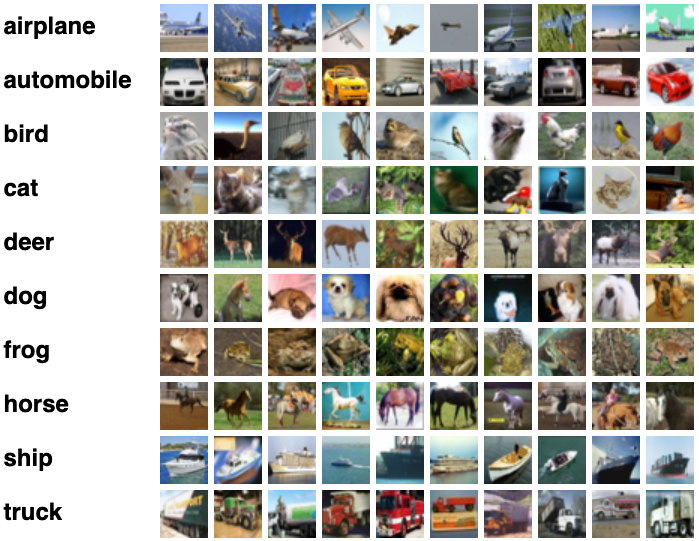
\includegraphics[width=\textwidth]{images/results/CIFAR_10.png}
    \centering
    \caption{CIFAR-10 sample images}\label{fig:CIFAR_10}
\end{figure}

The classes are completely mutually exclusive. There is no overlap between
automobiles and trucks. ``Automobile'' includes sedans, SUVs, things of that
sort. ``Truck'' includes only big trucks. Neither includes pick-up trucks.

\subsection{ImageNet 2012 dataset}
ImageNet is an image dataset organized according to the WordNet hierarchy. Each
meaningful concept in WordNet, possibly described by multiple words or word
phrases, is called a ``synonym set'' or ``synset''. There are more than 100000
synsets in WordNet, majority of them are nouns (80000+). In ImageNet, there are
on average 1000 images to illustrate each synset.
Images of each concept are quality-controlled and human-annotated. In its
completion, ImageNet will offer tens of millions of cleanly sorted images for
most of the concepts in the WordNet hierarchy (\autoref{fig:imagenet})

\begin{figure}[ht]
    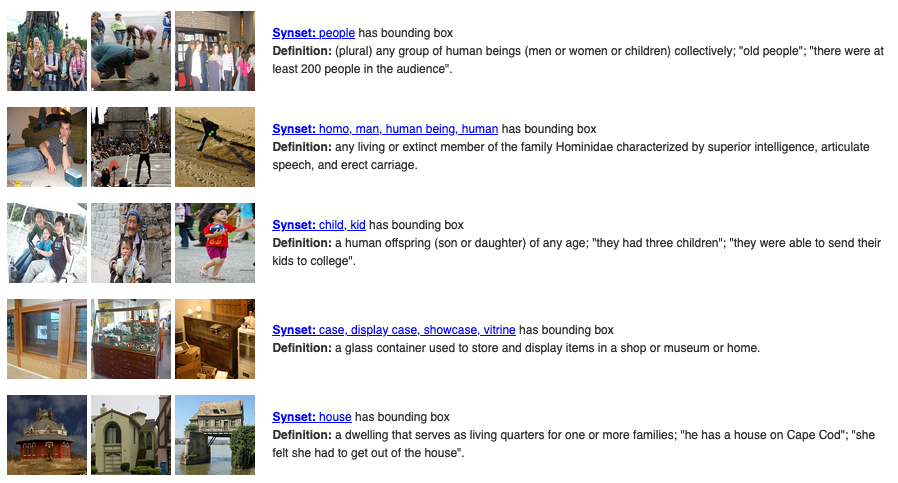
\includegraphics[width=\textwidth]{images/results/imagenet.png}
    \centering
    \caption{ImageNet sample images}\label{fig:imagenet}
\end{figure}

The dataset I've used for the experiments has the following sets:

\begin{itemize}
    \item \texttt{train} containing \textbf{1281167 images}
    \item \texttt{validation} containing \textbf{50000 images}
\end{itemize}

There supposed to be a \texttt{test} set but it doesn't have labels because no
labels have been publicly released.

The ILSVRC uses a ``trimmed'' list of only \textbf{1000 image categories} or
``classes'', including 90 of the 120 dog breeds classified by the full ImageNet
schema.

\section{Experiment results}
After a brief explanation of the model and the datasets used for the
experiments, in this section I show what results I have in pruning MobileNet v1
with CIFAR-10 and ImageNet.

\subsection{Environments}
The environment used for running CIFAR-10 experiments has the following
characteristics:

\begin{itemize}
    \item \textbf{CPU and memory:} 2 x Intel Xeon Gold 5120T CPU @ 2.20GHz, 28
        cores (56 threads) total, 64GB memory
    \item \textbf{Graphic:} NVIDIA TITAN Xp, 12GB GDDR5X, 3840 cores, CUDA
        driver version: 460.27.04, CUDA version: 11.2
    \item \textbf{Operating System:} Ubuntu 18.04.5 LTS, kernel
        5.4.0\-60-generic
    \item \textbf{Software Stack:} Python 3.8.5, TensorFlow 2.4.0, TFMOT
        0.5.0.dev20210206 with my patch for heuristic distribution, and
        dependencies. Everything has been isolated using conda
        (\url{https://docs.conda.io/en/latest/})
\end{itemize}

The environment used for running ImageNet experiments has the following
characteristics:

\begin{itemize}
    \item \textbf{CPU and memory:} AWS p3.2xlarge, 8 vCPU, 61GB memory
    \item \textbf{Graphic:} NVIDIA Tesla V100, 16GB, 5120 cores, CUDA Driver
        Version: 450.80.02, CUDA Version: 11.0
    \item \textbf{Operating System:} Ubuntu 18.04.5 LTS, kernel
        5.4.0\-1037-aws
    \item \textbf{Software Stack:} Python 3.7.6, TensorFlow 2.4.1, TFMOT
        0.5.0.dev20210206 with my patch for heuristic distribution, and
        dependencies. Everything has been isolated using conda
        (\url{https://docs.conda.io/en/latest/})
\end{itemize}

The reason I chose AWS for ImageNet is because of the time the training takes
with this dataset: one epoch is about 1.5h and I needed to run 20 epochs.
As I show later, the number of experiments are 20 and AWS gives me the
flexibility to have multiple instances in parallel.

\subsection{Pipeline details}
In order to run experiments, I've developed a custom pipeline (not included in
this thesis) which executes the following steps:

\begin{enumerate}
    \item Load in memory the model architecture from a pre-trained checkpoint
    \item Convert the model into float32, int8 and int16 tflite format
    \item Prune the original model with given parameters
    \item Check model sparsity and calculate loss, TOP-1 and TOP-5 accuracies
    \item Convert the pruned model into float32, int8 and int16 tflite format
    \item For every tflite generated, run:
    \begin{enumerate}
        \item Accuracy evaluation on the validation dataset (10000 samples)
        \item Get the size and compressed size of the tflite file
        \item Only for int8/int16 tflite files: run Ethos-U vela
            (\autoref{sub:vela}) to get an estimation of the inference speed on
            Ethos-U NPU and the tflite size of the vela generated tflite file.
    \end{enumerate}
\end{enumerate}

The above pipeline has been run passing different sparsity level and
distributions. I ran 10 pipelines for every dataset: (Heuristic, 0.5),
(Uniform, 0.5), (Heuristic, 0.75), (Uniform, 0.75), (Heuristic, 0.8),
(Uniform, 0.8), (Heuristic, 0.85), (Uniform, 0.85), (Heuristic, 0.9),
(Uniform, 0.9).

The pruning scheduler chosen is \texttt{PolynomialDecay}: sparsity is
introduced slowly, model weights can take into account this impact and become
robust to the effect of weights being dropped.

Every run of the pipeline gives the following metrics:
\begin{enumerate}
    \item Keras model: loss, TOP-1 and TOP-5 accuracies
    \item For every tflite file: sizes of the original model, compressed, and
        pruned compressed
    \item For every int8/int16 tflite file: inference speed and vela compressed
        size
\end{enumerate}

Later I'll show graph that compares the above metrics across sparsity levels
and distributions.

\subsection{Ethos-U Vela}\label{sub:vela}
Vela is a tool used to compile a TensorFlow Lite for Microcontroller (tflite)
neural network model into an optimised version that can run on an embedded
system containing an Arm Ethos-U NPU\@.

In order to be accelerated by the Ethos-U NPU the network operators must be
quantised to either 8-bit (unsigned or signed) or 16-bit (signed).

The optimised model will contain TensorFlow Lite Custom operators for those
parts of the model that can be accelerated by the Ethos-U NPU\@. Parts of the
model that cannot be accelerated are left unchanged and will instead run on the
Cortex-M series CPU using an appropriate kernel (such as the Arm optimised
CMSIS-NN kernels).

After compilation the optimised model can only be run on an Ethos-U NPU
embedded system.

The tool will also generate performance estimates for the compiled model.

For more information about vela, please refer to PyPi home page
\url{https://pypi.org/project/ethos-u-vela/}

\subsubsection{Vela memory optimization}\label{subsub:vela_memory_optimization}
The Vela compiler also performs various memory optimizations to reduce both the
permanent (for example flash) and runtime (for example SRAM) memory
requirements.
One such technique for permanent storage is the compression of all the weights
in the model.

Another technique is cascading, which addresses the runtime memory usage.
Cascading reduces the maximum memory requirement by splitting the feature maps
(FM) of a group of consecutively supported operators into stripes. A stripe can
be either the full or partial width of the FM\@. And it can be the full or
partial height of the FM\@. Each stripe in turn is then run through all the
operators in the group.

The parts of the model that can be optimized and accelerated are grouped and
converted into TensorFlow Lite custom operators. The operators are then
compiled into a command stream that can be executed by the Ethos-U NPU\@.

Finally, the optimized model is written out as a $TFL\mu$ model and a
Performance Estimation report is generated that provides statistics, such as
memory usage and inference time.

The compiler includes numerous configuration options that allow you to specify
various aspects of the embedded system configuration (for example the Ethos-U
NPU configuration, memory types, and memory sizes). There are also options to
control the types of optimization that are performed during the compilation
process.\cite{vela_compiler}

\subsection{Results for MobileNet v1 with CIFAR-10}
For running this experiment the classical MobileNet v1 architecture has been
slightly modified on three layers.

\begin{figure}[ht]
    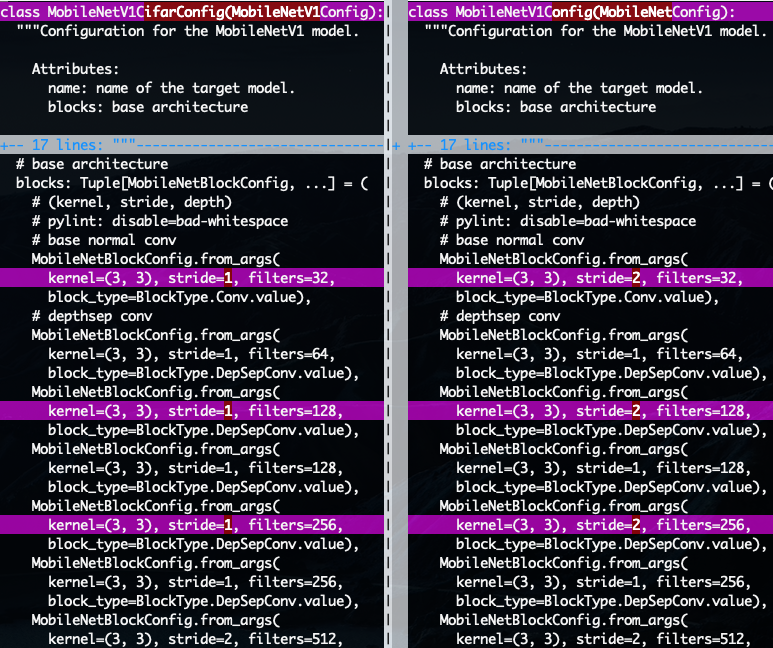
\includegraphics[width=9cm]{images/results/mobilenet_cifar10_diff.png}
    \centering
    \caption{MobileNet v1 changes for CIFAR-10}\label{fig:mobilenet_cifar10_diff}
\end{figure}

The original MobileNet architecture is designed for ImageNet dataset where
images' size is $224\times224\times3$. Because CIFAR-10 images have smaller
size ($32\times32$) I had to modify slightly the architecture.

The main change is that in the first layers the \texttt{stride=2} has been
replaced with \texttt{stride=1}.
\autoref{fig:mobilenet_cifar10_diff} shows what the difference is between
MobileNet for CIFAR-10 and the classical architecture.

The fine-tuning of the model has been done with the following hyper parameters
which have been found with Keras Tuner
(\url{https://keras-team.github.io/keras-tuner/}):

\begin{itemize}
    \item \textbf{Optimizer}: SGD (Stochastic Gradient Descend)
    \item \textbf{Optimizer momentum}: 0
    \item \textbf{Batch size}: 32
    \item \textbf{Learning rate}: 6.995e-06 (0.000006995)
    \item \textbf{Epochs}: 15
    \item \textbf{Sparsity scheduler}: Polynomial Decay
\end{itemize}

\subsubsection{Accuracy and loss results}
In this section I analyse data about accuracy and loss. The heuristic
distribution will be always compared to the uniform distribution.

For reference, \textbf{the TOP-1 accuracy of a non-pruned MobileNet v1 with
CIFAR-10 is 0.9487.}

\autoref{fig:cifar10_top1_top5_loss} shows how the two distributions impact the
TOP-1/TOP-5 accuracies and the loss function.

\begin{figure}
    \centering
    {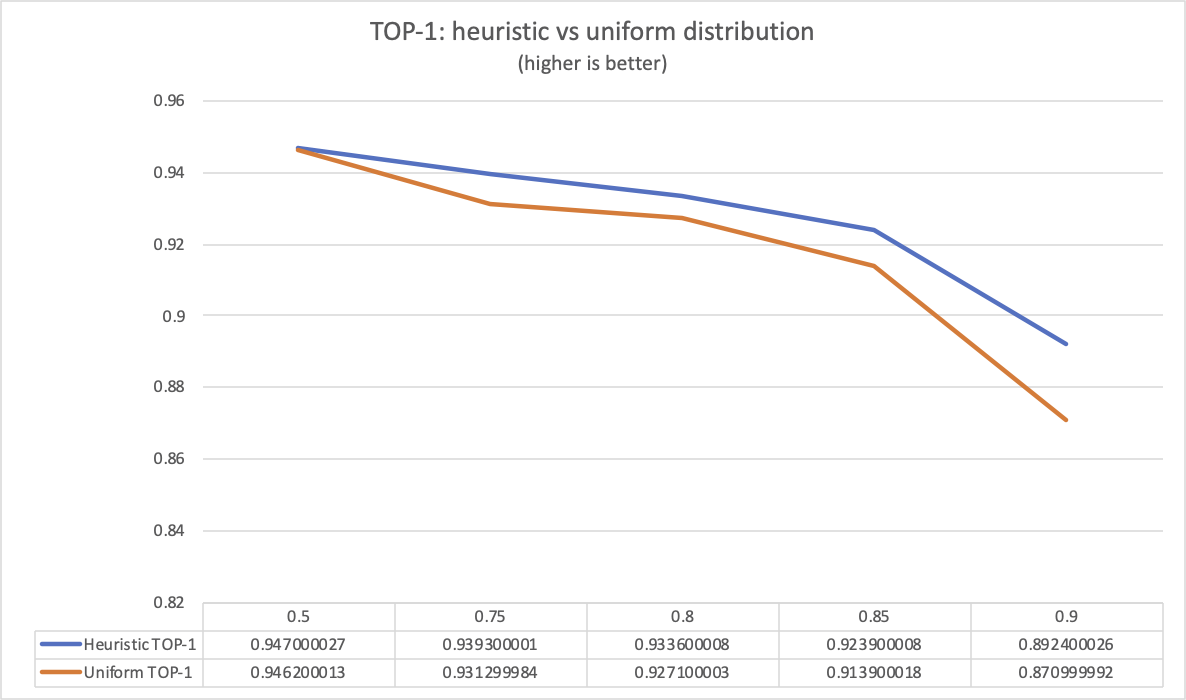
\includegraphics[width=.85\linewidth]{images/results/cifar10_top1.png}}
    {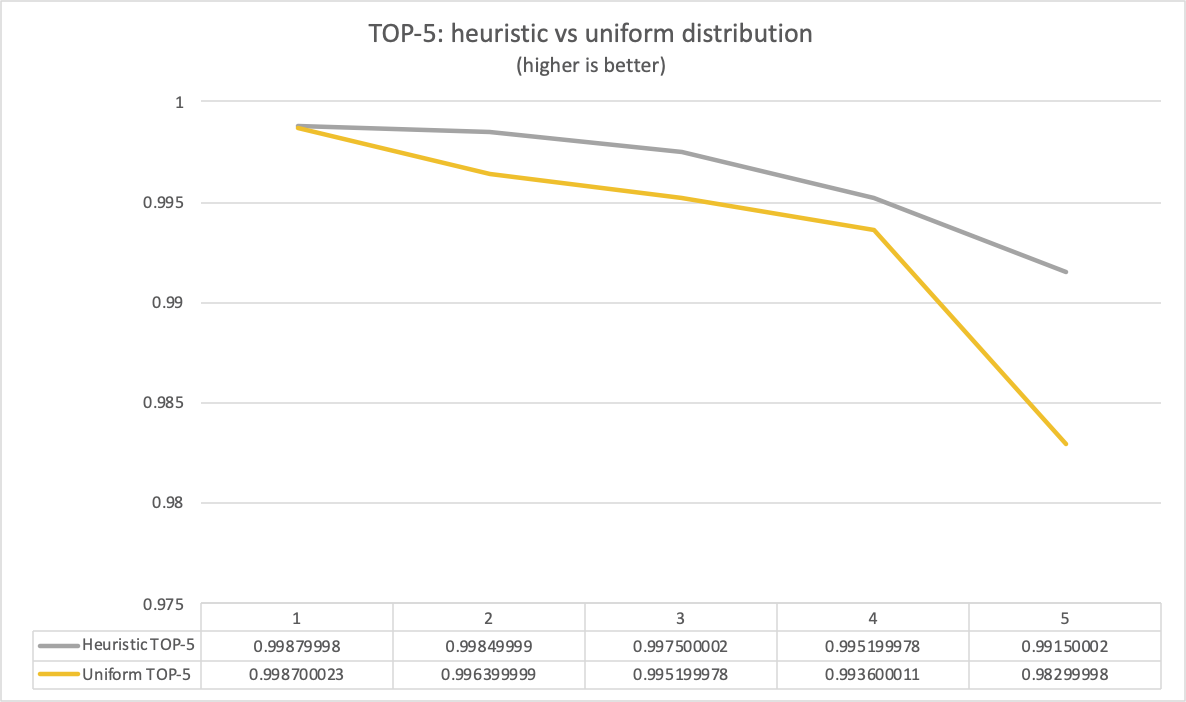
\includegraphics[width=.85\linewidth]{images/results/cifar10_top5.png}}
    {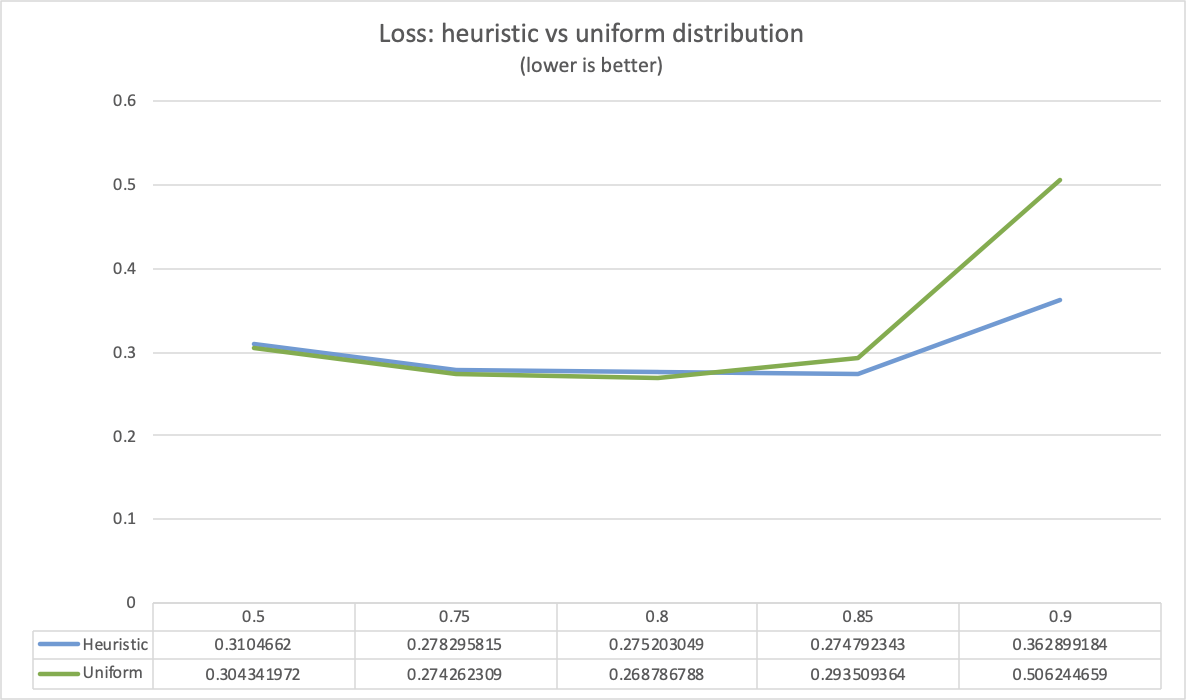
\includegraphics[width=.85\linewidth]{images/results/cifar10_loss.png}}
    \caption{Heuristic vs Uniform: CIFAR-10 TOP-1/TOP-5 and Loss}\label{fig:cifar10_top1_top5_loss}
\end{figure}

The first thing to notice is that the heuristic distribution always outperforms
the uniform distribution both for TOP-1 (blue line) and TOP-5 (grey line).
The heuristic distribution seems more robust compared to the uniform and this
is highlighted by the fact it loses less in accuracy when the sparsity is
increasing.
When the sparsity is set to 0.9, the heuristic distribution has an increase of
\textbf{2.14\% in the TOP-1} compared to the uniform distribution.
A sweet spot though is at \textbf{sparsity 0.85}: the model doesn't lose too
much accuracy compared to its non-pruned baseline and the sparsity is high
enough to see benefits in terms of size, memory and latency of the inference.
At this sparsity level, the heuristic distributions gains 1\% in accuracy
compared to the uniform distribution, giving an accuracy of \textbf{0.9239\%}:
this is \textbf{only 2.48\% less} than the non-pruned accuracy.

The loss has a slightly different trend: up to a sparsity level of 0.8, there
is no big difference between the two distributions with the uniform being
slightly better.
The trend completely flips at the latest two highest sparsity level: the loss
of the uniform distribution increases much more compared to the heuristic one.
This is another proof that the heuristic distribution seems more robust at
higher sparsity levels.

\begin{figure}[ht]
    \centering
    {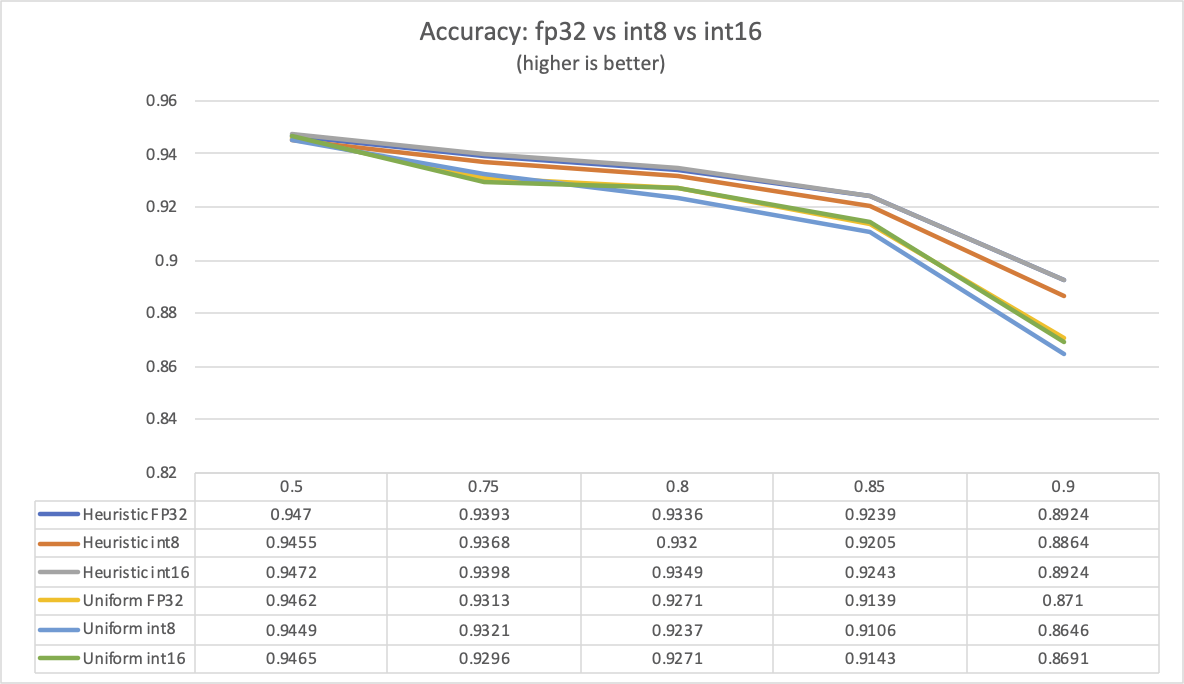
\includegraphics[width=.8\linewidth]{images/results/cifar10_tflite_accuracy.png}}
    \caption{Heuristic vs Uniform: CIFAR-10 tflite accuracy}\label{fig:cifar10_tflite_accuracy}
\end{figure}

\autoref{fig:cifar10_tflite_accuracy} shows accuracy across FP32, int8 and
int16 tflite models both for uniform and heuristic distribution.

This graph confirms the trend seen in the previous ones: independently of the
quantization scheme used, \textbf{the heuristic distribution performs better
than the uniform one across all sparsity levels}.
The top 3 lines (dark blue, amber and grey) represent the accuracies of the
heuristic distribution whilst the bottom 3 lines (yellow, light blue and green)
represent the accuracies of the uniform distribution.
Moreover the heuristic distribution seems to have a smoother trend across
sparsity levels compared to the uniform distribution.

\subsubsection{tflite size results}\label{subsub:tflite_size_results}
\autoref{fig:cifar10_tflite_size} shows the sizes of tflite files across
different sparsity levels for FP32, int8 and int16.

\begin{figure}[ht]
    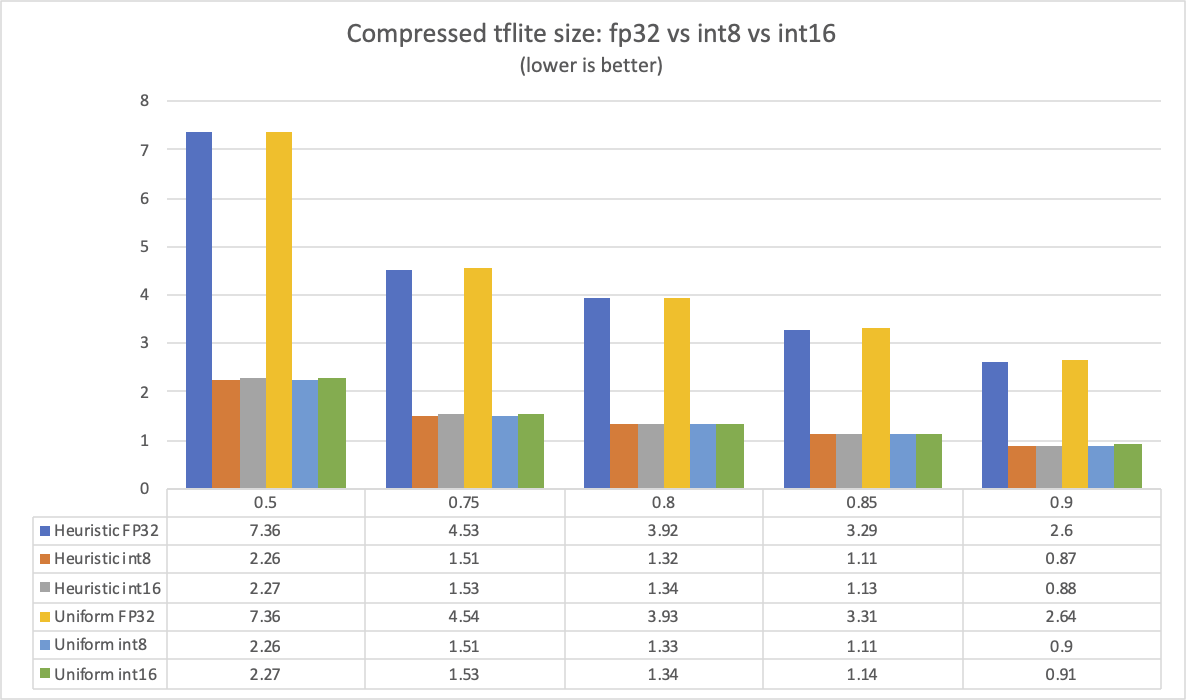
\includegraphics[width=\linewidth]{images/results/cifar10_tflite_size.png}
    \centering
    \caption{Heuristic vs Uniform: CIFAR-10 FP32, int8, int16 tflite size}\label{fig:cifar10_tflite_size}
\end{figure}

The sparsity distribution doesn't really influence the size of the tflite:
the distribution controls how weights are distributed across layers while
maintaining the final sparsity of the model. \textbf{The number of weights is
exactly the same.}
As example let's take the 0.85 sparsity level and see how the weights are
distributed in both heuristic and uniform distribution.

\begin{lstlisting}[label={lst:heuristic_weights_cifar10},
    caption=MobileNet v1 and CIFAR-10: heuristic weights distributions]
Conv2d_0_0:            864 weights,     384 zero weights,    0.4444444444444444 sparsity
Conv2d_1/pointwise:    2048 weights,    1026 zero weights,   0.5009765625 sparsity
Conv2d_2/pointwise:    8192 weights,    4851 zero weights,   0.5921630859375 sparsity
Conv2d_3/pointwise:    16384 weights,   10448 zero weights,  0.6376953125 sparsity
Conv2d_4/pointwise:    32768 weights,   22388 zero weights,  0.6832275390625 sparsity
Conv2d_5/pointwise:    65536 weights,   47760 zero weights,  0.728759765625 sparsity
Conv2d_6/pointwise:    131072 weights,  101490 zero weights, 0.7743072509765625 sparsity
Conv2d_7/pointwise:    262144 weights,  214920 zero weights, 0.819854736328125 sparsity
Conv2d_8/pointwise:    262144 weights,  214920 zero weights, 0.819854736328125 sparsity
Conv2d_9/pointwise:    262144 weights,  214920 zero weights, 0.819854736328125 sparsity
Conv2d_10/pointwise:   262144 weights,  214920 zero weights, 0.819854736328125 sparsity
Conv2d_11/pointwise:   262144 weights,  214920 zero weights, 0.819854736328125 sparsity
Conv2d_12/pointwise:   524288 weights,  453721 zero weights, 0.8654041290283203 sparsity
Conv2d_13/pointwise:   1048576 weights, 955202 zero weights, 0.9109516143798828 sparsity
top/Conv2d_1x1_output: 10250 weights,   6213 zero weights,   0.6061463414634146 sparsity
Sparse weights: 2678083
All weights: 3150698
Overall model sparsity: 0.8499967309
\end{lstlisting}

As shown in \autoref{lst:heuristic_weights_cifar10}, the heuristic distribution
of the weights has set to zero about 91\% of the weights in the layer
\texttt{Conv2d\_13/pointwise} while the first layers of the model have a
sparsity below 50\%.

For reference, \autoref{lst:uniform_weights} shows the same sparsity level
(0.85) but with a uniform distribution. All layers have 85\% of the weights set
to zero.

\begin{lstlisting}[label={lst:uniform_weights},
    caption=MobileNet v1 and CIFAR-10: uniform weights distributions]
Conv2d_0_0:            864 weights,    734 zero weights,    0.8495370370370371 sparsity
Conv2d_1/pointwise:    2048 weights,   1741 zero weights,   0.85009765625 sparsity
Conv2d_2/pointwise:    8192 weights,   6963 zero weights,   0.8499755859375 sparsity
Conv2d_3/pointwise:    16384 weights,  13926 zero weights,  0.8499755859375 sparsity
Conv2d_4/pointwise:    32768 weights,  27853 zero weights,  0.850006103515625 sparsity
Conv2d_5/pointwise:    65536 weights,  55706 zero weights,  0.850006103515625 sparsity
Conv2d_6/pointwise:    131072 weights, 111411 zero weights, 0.8499984741210938 sparsity
Conv2d_7/pointwise:    262144 weights, 222822 zero weights, 0.8499984741210938 sparsity
Conv2d_8/pointwise:    262144 weights, 222822 zero weights, 0.8499984741210938 sparsity
Conv2d_9/pointwise:    262144 weights, 222822 zero weights, 0.8499984741210938 sparsity
Conv2d_10/pointwise:   262144 weights, 222822 zero weights, 0.8499984741210938 sparsity
Conv2d_11/pointwise:   262144 weights, 222822 zero weights, 0.8499984741210938 sparsity
Conv2d_12/pointwise:   524288 weights, 445645 zero weights, 0.8500003814697266 sparsity
Conv2d_13/pointwise:   1048576 weights,891290 zero weights, 0.8500003814697266 sparsity
top/Conv2d_1x1_output: 10250 weights,  8704 zero weights,   0.849170731707317 sparsity
Sparse weights: 2678083
All weights: 3150698
Overall model sparsity: 0.8499967309
\end{lstlisting}

What the \autoref{fig:cifar10_tflite_size} highlights though is that quantized
models have a much smaller size compared to FP32.

As reference, the uncompressed version of the tflite files are:
\begin{itemize}
    \item \textbf{FP32}: 12.85Mb
    \item \textbf{int8}: 3.61Mb
    \item \textbf{int16}: 3.65Mb
\end{itemize}

At 0.85 sparsity level, there are the following gains in terms of sizes:
\begin{itemize}
    \item \textbf{FP32}: 12.85Mb $\rightarrow$ 3.30Mb, a \textbf{decrease of 74.31\%}
    \item \textbf{int8}: 3.61Mb $\rightarrow$ 1.11Mb, a \textbf{decrease of 69.25\%}
    \item \textbf{int16}: 3.65Mb $\rightarrow$ 1.13, a \textbf{decrease of 69.04\%}
\end{itemize}

As mentioned in \autoref{subsub:vela_memory_optimization}, vela compiler has a
compression mechanism built it when parsing a tflite file. In fact vela
generates a new tflite file which has a better compression rate compared to
gzip. Let's take the above sparsity level (0.85) and see how vela compiler
affects the tflite size. Of course this is true \textbf{only for quantized
tflite models.}
The non pruned quantized models (both int8 and int16) have a \textbf{vela size
of 3Mb.}. The pruned ones have a \textbf{vela size of 0.91Mb}, a \textbf{a
decrease of 69.67\%}.

Let's take the 2 extreme points of the tflite sizes: FP32 non pruned and
int8/int16 pruned at 0.85. \textbf{The tflite size goes from 12.85 to 0.91Mb,
a decrease of 92.92\%}. The accuracy goes from 0.9487 to 0.9205
(int8) or 0.9243 (int16), \textbf{a decrease of 2.97\% (int8) or 2.57\% (int16)}

\subsubsection{Inference speed results (int8 and int16 only)}
The inference speed showed in \autoref{fig:cifar10_inf_speed} are generated by
vela while optimising the tflite file. Vela compiler can take multiple profiles
depending for what NPU it needs to optimise the tflite for.

\begin{figure}
    \centering
    \subcaptionbox{Inference speed}
    {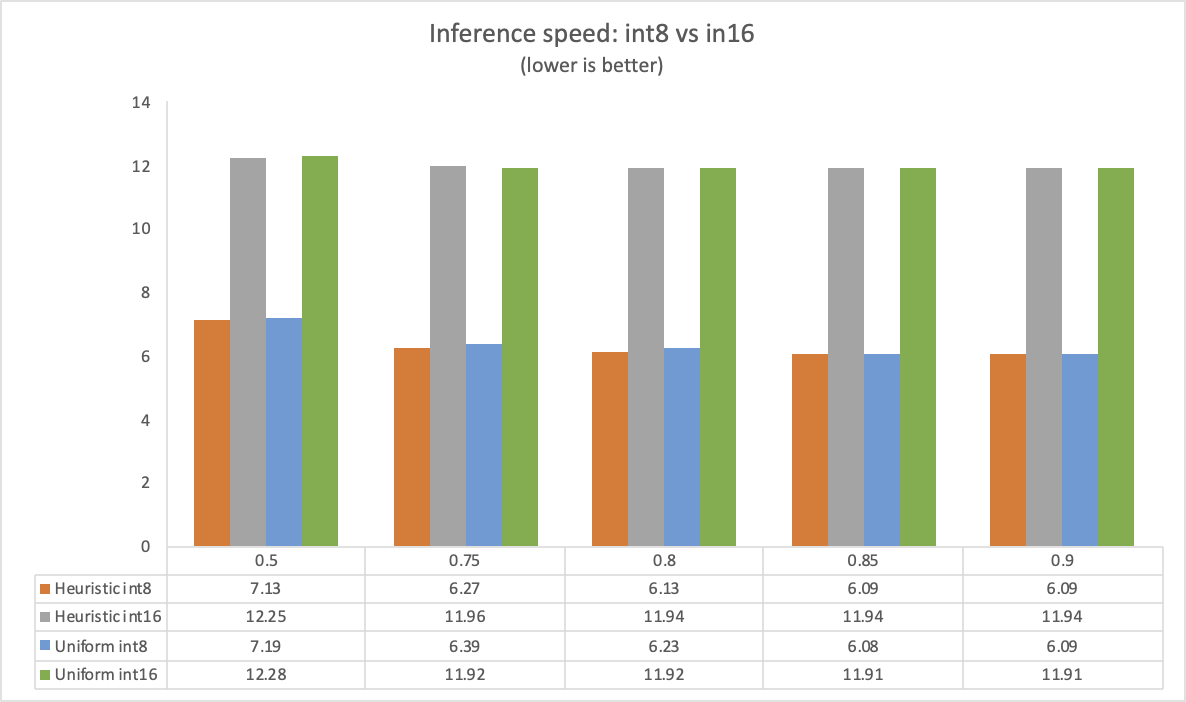
\includegraphics[width=1\linewidth]{images/results/cifar10_inf_speed.png}}
    \subcaptionbox{Inferences per second}
    {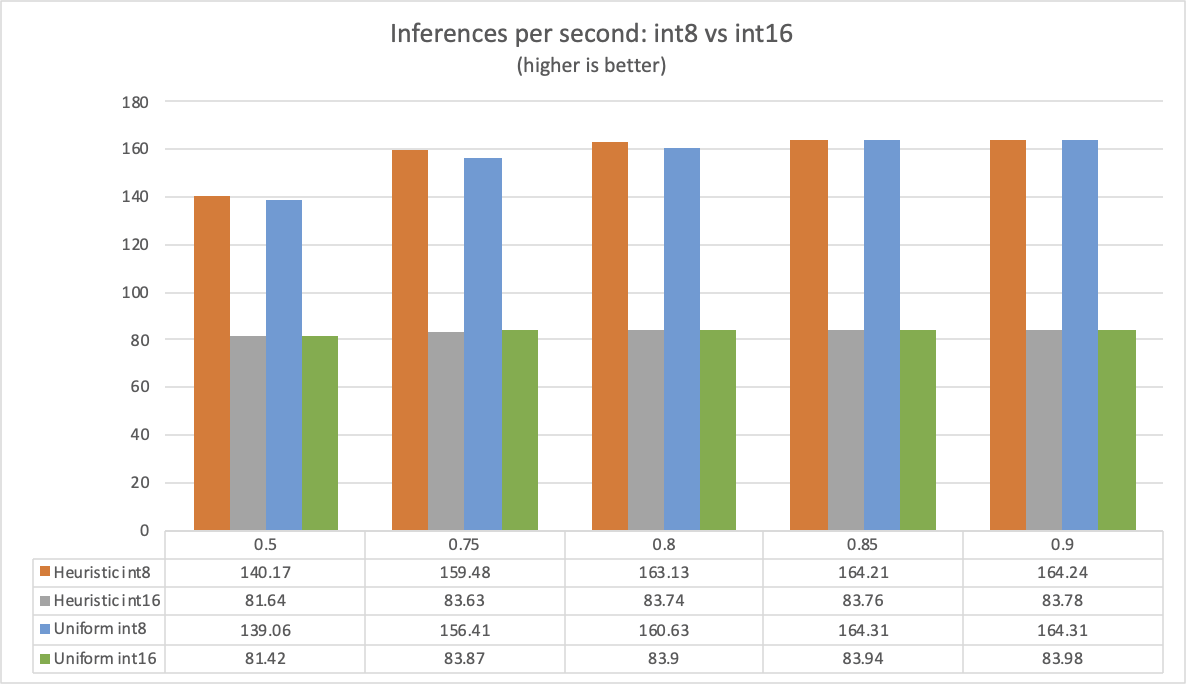
\includegraphics[width=1\linewidth]{images/results/cifar10_infs_second.png}}
    \caption{Heuristic vs Uniform: CIFAR-10 int8, int16 inference speed}\label{fig:cifar10_inf_speed}
\end{figure}

In this case the it has been optimised for an Ethos-U55 high-end embedded NPU
with the following characteristics: SRAM, 4 GB/s and flash, 0.5 GB/s.
\autoref{lst:vela_output_cifar10} shows vela output with estimations. At the very end
there is the inference speed (\texttt{Batch Inference time})

\begin{lstlisting}[label={lst:vela_output_cifar10},
    caption=MobileNet v1 and CIFAR-10: vela output on an int8 tflite file]
Warning: Using internal-default values for memory mode
Info: MEAN model_2/top/GlobalPool/Mean is a CPU only op
Warning: Mean operation is unknown or unsupported, placing on CPU

Network summary for mobilenet-v1_cifar10-int8-pruned
Accelerator configuration               Ethos_U55_256
System configuration             Ethos_U55_High_End_Embedded
Memory mode                          internal-default
Accelerator clock                                 500 MHz
Design peak SRAM bandwidth                       4.00 GB/s
Design peak Off-chip Flash bandwidth             0.50 GB/s

Total SRAM used                                415.64 KiB
Total Off-chip Flash used                      899.83 KiB (2.20 bits per element)

69 passes fused into 58
1/191 (52.4%) operations falling back to the CPU
Average SRAM bandwidth                           2.82 GB/s
Input   SRAM bandwidth                           7.71 MB/batch
Weight  SRAM bandwidth                           6.19 MB/batch
Output  SRAM bandwidth                           3.25 MB/batch
Total   SRAM bandwidth                          17.19 MB/batch
Total   SRAM bandwidth            per input     17.19 MB/inference (batch size 1)

Average Off-chip Flash bandwidth                 0.14 GB/s
Input   Off-chip Flash bandwidth                 0.11 MB/batch
Weight  Off-chip Flash bandwidth                 0.77 MB/batch
Output  Off-chip Flash bandwidth                 0.00 MB/batch
Total   Off-chip Flash bandwidth                 0.88 MB/batch
Total   Off-chip Flash bandwidth  per input      0.88 MB/inference (batch size 1)

Neural network macs                         611565578 MACs/batch
Hardware macs                               668484736 MACs/batch
Network Tops/s                                   0.20 Tops/s
Hardware Tops/s                                  0.22 Tops/s

NPU cycles                                    2967787 cycles/batch
SRAM Access cycles                            2148562 cycles/batch
DRAM Access cycles                                  0 cycles/batch
On-chip Flash Access cycles                         0 cycles/batch
Off-chip Flash Access cycles                   881088 cycles/batch
Total cycles                                  3044776 cycles/batch

Batch Inference time                 6.09 ms,  164.22 inferences/s (batch size 1)
\end{lstlisting}

Similarly to what has been observed in \autoref{subsub:tflite_size_results},
the distribution doesn't really impact the inference speed.
It looks like though that the heuristic distributions is slightly faster than
the uniform one but the increase is so small that can be ignored.

\autoref{fig:cifar10_inf_speed} shows anyway that int16 is much slower than
int8: this because the native MACs (multiply-accumulate) operations in
Ethos-U55 are 8 (for weights) $\times$ 8 (for activations) bit.
8$\times$16-bit operations run at half the speed of 8$\times$8-bit
operations as a 8$\times$16 MAC is twice as complex as an 8$\times$8 MAC\@.

Let's take the inference time for non-pruned tflite files and see what kind of
speed up there is with a pruned model at 0.85.

\begin{itemize}
    \item \textbf{int8}: 8.68ms $\rightarrow$ 6.09ms, a \textbf{decrease of 29.84\%}
    \item \textbf{int16}: 13.93ms $\rightarrow$ 11.91ms, a \textbf{decrease of 14.50\%}
\end{itemize}

Quantization has a huge benefit in terms of tflite size and latency of the
inference and the benefits are even bigger when paired up with pruning.

\subsection{Results MobileNet v1 with ImageNet 2012}
After seen the results using CIFAR-10, in this section the dataset used is
ILSVRC (ImageNet Large Scale Visual Recognition Challenge) 2012, commonly known
as ImageNet.

There are no architectural changes to the model.

The fine-tuning of the model has been done with the following hyper parameters
found via experimentations:

\begin{itemize}
    \item \textbf{Optimizer}: SGD (Stochastic Gradient Descend)
    \item \textbf{Optimizer momentum}: 0.9
    \item \textbf{Optimizer decay rate}: 0.9
    \item \textbf{Learning rate decay rate}: 0.94
    \item \textbf{Learning rate decay epochs}: 2.5
    \item \textbf{Dropout rate}: 0.2
    \item \textbf{Standard weight decay}: 4e-05
    \item \textbf{Truncated normal standard deviation}: 0.09
    \item \textbf{Batch norm decay}: 0.9997
    \item \textbf{Batch size}: 64
    \item \textbf{Learning rate}: 0.001
    \item \textbf{Epochs}: 20
    \item \textbf{Sparsity scheduler}: Polynomial Decay
\end{itemize}

\subsubsection{Accuracy and loss results}
For ImageNet I focus mainly on the FP32 results as similar considerations to
CIFAR-10 can be done for quantized models in terms of accuracy.

Like before, the heuristic distribution will be always compared to the uniform
distribution.

For reference, \textbf{the TOP-1 accuracy of a non-pruned MobileNet v1 with
ImageNet is 0.709.}

\autoref{fig:imagenet_top1_top5_loss} shows how the two distributions impact the
TOP-1/TOP-5 accuracies and the loss function.

\begin{figure}
    \centering
    {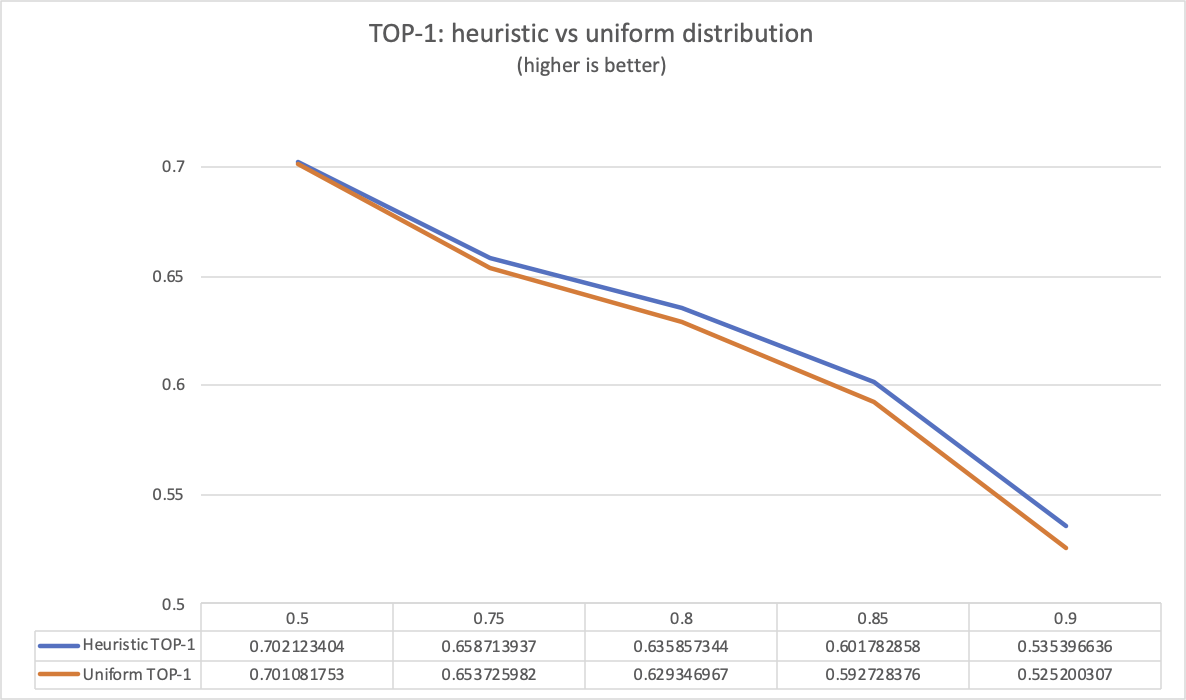
\includegraphics[width=.85\linewidth]{images/results/imagenet_top1.png}}
    {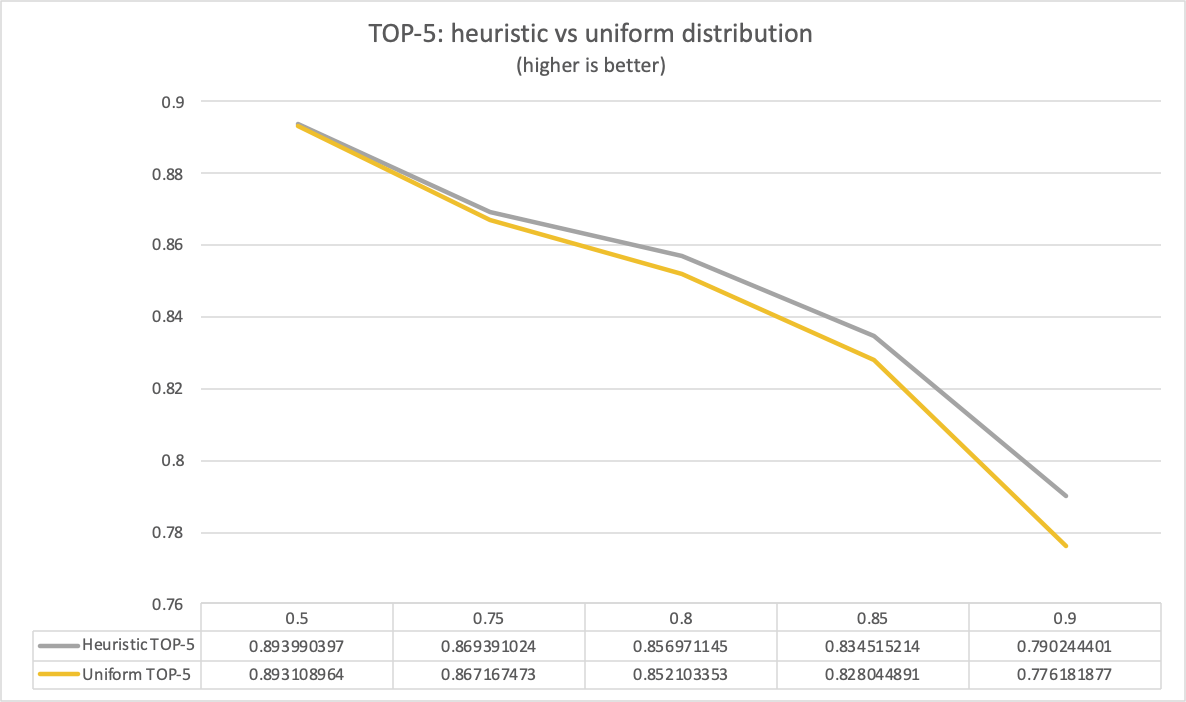
\includegraphics[width=.85\linewidth]{images/results/imagenet_top5.png}}
    {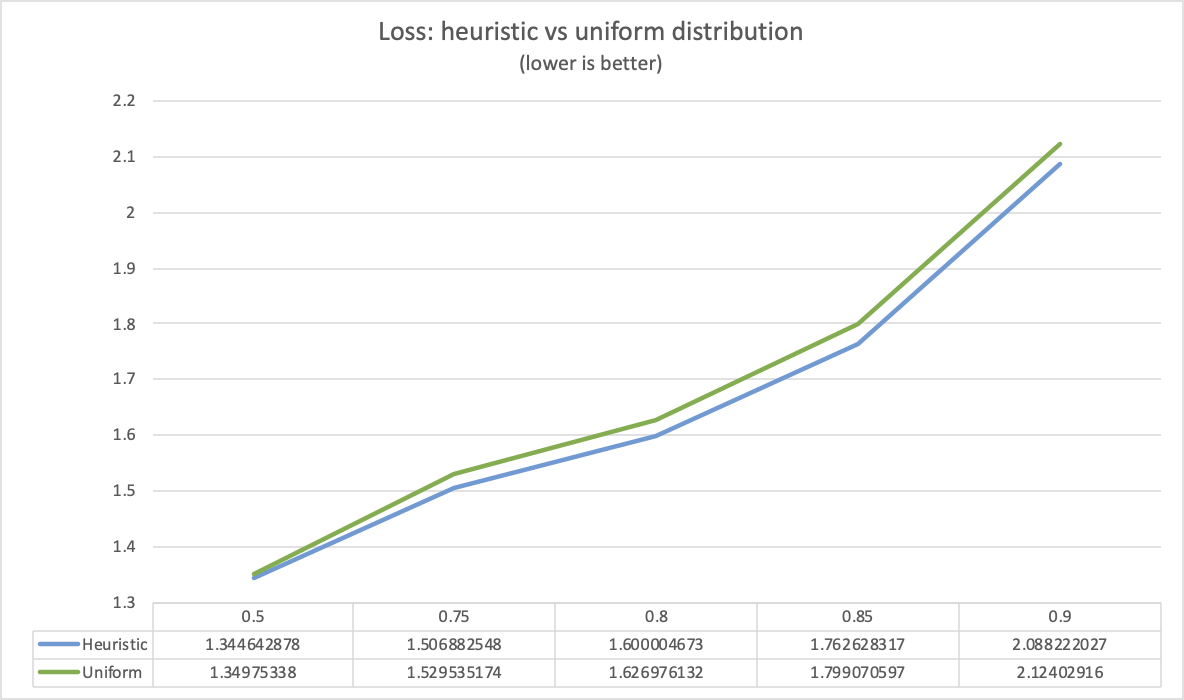
\includegraphics[width=.85\linewidth]{images/results/imagenet_loss.png}}
    \caption{Heuristic vs Uniform: ImageNet TOP-1/TOP-5 and Loss}\label{fig:imagenet_top1_top5_loss}
\end{figure}

Like in the previous case, the heuristic distribution always outperforms the
uniform distribution both for TOP-1 (blue line) and TOP-5 (grey line).
The heuristic distribution seems more a little bit more robust compared to the
uniform one as the sparsity increases the difference between the two sparsity
increases slightly.
When the sparsity is set to 0.9, the heuristic distribution has an increase of
\textbf{1.02\% in the TOP-1} compared to the uniform distribution.
\textbf{Any sparsity bigger than 0.5 is going to have an impact in terms of
accuracy}: the TOP-1 accuracy for a non pruned model is 0.709 and for a
sparsity of 0.5 there is a TOP-1 accuracy of 0.7021 for the heuristic
distribution and 0.7011 for the uniform distribution.
If the requirements of the application need to have a close accuracy of the
original model, then 0.5 is a pretty good sparsity level. At this point
choosing one of the other distribution changes very little in terms of
accuracy: the heuristic has only \textbf{0.1041\%} more accuracy than the
uniform distribution.
If the application requires a smaller model, it needs to compromise in the
accuracy: from 0.75 to 0.85 sparsity level, there is a drop of about 6\%.
At 0.85 sparsity level, the heuristic distribution has an accuracy of
\textbf{0.6018} whilst the uniform distributions falls in the range below, at
\textbf{0.5927}.
At 0.9 sparsity level there is a steeper drop in accuracy (around 0.52): with
this accuracy it might not make any sense to deploy the model at all.
If the sparsity needs to be between 0.5 and 0.85 then the heuristic
distribution is the one of choice as it gives better accuracy.

The loss follows has a specular behaviour of the TOP-1 accuracy: at 0.5
sparsity level the loss function is the same for both distribution.
From 0.75 to 0.85 they increase almost in a parallel fashion and to get to 0.9
were both distributions have a steeper increase.
Anyway from 0.75 to 0.9 the heuristic distribution (blue line) has always a
smaller loss function compared to the uniform.
This is another proof that the heuristic distribution seems more robust at
higher sparsity levels.

\subsubsection{tflite size results}
Like in the previous case, the sparsity distribution doesn't really influence
the size of the tflite: the number of weights is exactly the same between the
uniform and the heuristic distributions.

This model though is bigger than the previous one: even the architecture is the
same, it deals with different input size: CIFAR-10 images are 32$\times$32
whilst ImageNet images are 224$\times$224.

Let's take the 0.85 sparsity level and see how the weights are distributed
following the heuristic distribution.

\begin{lstlisting}[label={lst:heuristic_weights_imagenet},
    caption=MobileNet v1 and ImageNet: heuristic weights distributions]
2021-02-19 15:26:23,484 Conv2d_0_0:            864 weights,     377 zero weights,    0.4363425925925926 sparsity
2021-02-19 15:26:23,488 Conv2d_1/pointwise:    2048 weights,    1008 zero weights,   0.4921875 sparsity
2021-02-19 15:26:23,492 Conv2d_2/pointwise:    8192 weights,    4765 zero weights,   0.5816650390625 sparsity
2021-02-19 15:26:23,496 Conv2d_3/pointwise:    16384 weights,   10264 zero weights,  0.62646484375 sparsity
2021-02-19 15:26:23,500 Conv2d_4/pointwise:    32768 weights,   21993 zero weights,  0.671173095703125 sparsity
2021-02-19 15:26:23,504 Conv2d_5/pointwise:    65536 weights,   46919 zero weights,  0.7159271240234375 sparsity
2021-02-19 15:26:23,508 Conv2d_6/pointwise:    131072 weights,  99704 zero weights,  0.76068115234375 sparsity
2021-02-19 15:26:23,512 Conv2d_7/pointwise:    262144 weights,  211138 zero weights, 0.8054275512695312 sparsity
2021-02-19 15:26:23,517 Conv2d_8/pointwise:    262144 weights,  211138 zero weights, 0.8054275512695312 sparsity
2021-02-19 15:26:23,522 Conv2d_9/pointwise:    262144 weights,  211138 zero weights, 0.8054275512695312 sparsity
2021-02-19 15:26:23,526 Conv2d_10/pointwise:   262144 weights,  211138 zero weights, 0.8054275512695312 sparsity
2021-02-19 15:26:23,531 Conv2d_11/pointwise:   262144 weights,  211138 zero weights, 0.8054275512695312 sparsity
2021-02-19 15:26:23,536 Conv2d_12/pointwise:   524288 weights,  445735 zero weights, 0.8501720428466797 sparsity
2021-02-19 15:26:23,543 Conv2d_13/pointwise:   1048576 weights, 938389 zero weights, 0.8949174880981445 sparsity
2021-02-19 15:26:23,547 top/Conv2d_1x1_output: 1026025 weights, 915809 zero weights, 0.8925796155064448 sparsity
2021-02-19 15:26:23,547 Sparse weights: 3540653
2021-02-19 15:26:23,547 All weights: 4166473
2021-02-19 15:26:23,547 Overall model sparsity: 0.849796218528237
\end{lstlisting}

As shown in \autoref{lst:heuristic_weights_imagenet}, the heuristic
distribution of the weights has set different sparsity levels for every layer
depending on how many weights a layer has.

As reference, the uncompressed version of the tflite files are:
\begin{itemize}
    \item \textbf{FP32}: 16.91Mb
    \item \textbf{int8}: 4.66Mb
    \item \textbf{int16}: 4.71Mb
\end{itemize}

At 0.85 sparsity level, there are the following gains in terms of sizes:
\begin{itemize}
    \item \textbf{FP32}: 16.91Mb $\rightarrow$ 4.07Mb, a \textbf{decrease of 75.93\%}
    \item \textbf{int8}: 4.66Mb $\rightarrow$ 1.43Mb, a \textbf{decrease of 69.31\%}
    \item \textbf{int16}: 4.71Mb $\rightarrow$ 1.13, a \textbf{decrease of 76.01\%}
\end{itemize}

The non pruned quantized models (both int8 and int16) have a \textbf{vela size
of 3.96Mb.}. The pruned ones have a \textbf{vela size of 1.16Mb}, a \textbf{a
decrease of 71.46\%}.

Let's take the 2 extreme points of the tflite sizes: FP32 non pruned and
int8/int16 pruned at 0.85. \textbf{The tflite size goes from 16.91 to 1.16Mb,
a decrease of 93.14\%}.

\subsubsection{Inference speed results (int8 and int16 only)}
Like in the previous, I have run vela for every experiment and the same
conclusions can be made: the distribution doesn't really impact the inference
speed.
It looks like though that the heuristic distributions is slightly faster than
the uniform one but the increase is so small that can be ignored.

Let's take the inference time for non-pruned tflite files and see what kind of
speed up there is with a pruned model at 0.85 (as shown in
\autoref{lst:vela_output_imagenet})

\begin{lstlisting}[label={lst:vela_output_imagenet},
    caption=MobileNet v1 and ImageNet: vela output on an int8 tflite file]
Info: MEAN model_2/top/GlobalPool/Mean is a CPU only op
Warning: Mean operation is unknown or unsupported, placing on CPU

Network summary for mobilenet-v1_imagenet2012-int8-pruned
Accelerator configuration               Ethos_U55_256
System configuration             Ethos_U55_High_End_Embedded
Memory mode                          internal-default
Accelerator clock                                 500 MHz
Design peak SRAM bandwidth                       4.00 GB/s
Design peak Off-chip Flash bandwidth             0.50 GB/s

Total SRAM used                                599.80 KiB
Total Off-chip Flash used                     1130.38 KiB (2.11 bits per element)

69 passes fused into 63
1/187 (53.5%) operations falling back to the CPU
Average SRAM bandwidth                           2.69 GB/s
Input   SRAM bandwidth                           9.77 MB/batch
Weight  SRAM bandwidth                           6.40 MB/batch
Output  SRAM bandwidth                           5.06 MB/batch
Total   SRAM bandwidth                          21.24 MB/batch
Total   SRAM bandwidth            per input     21.24 MB/inference (batch size 1)

Average Off-chip Flash bandwidth                 0.14 GB/s
Input   Off-chip Flash bandwidth                 0.12 MB/batch
Weight  Off-chip Flash bandwidth                 0.99 MB/batch
Output  Off-chip Flash bandwidth                 0.00 MB/batch
Total   Off-chip Flash bandwidth                 1.12 MB/batch
Total   Off-chip Flash bandwidth  per input      1.12 MB/inference (batch size 1)

Neural network macs                         568749545 MACs/batch
Hardware macs                               677312576 MACs/batch
Network Tops/s                                   0.14 Tops/s
Hardware Tops/s                                  0.17 Tops/s

NPU cycles                                    3812208 cycles/batch
SRAM Access cycles                            2655593 cycles/batch
DRAM Access cycles                                  0 cycles/batch
On-chip Flash Access cycles                         0 cycles/batch
Off-chip Flash Access cycles                  1115488 cycles/batch
Total cycles                                  3946734 cycles/batch

Batch Inference time                 7.89 ms,  126.69 inferences/s (batch size 1)
\end{lstlisting}


\begin{itemize}
    \item \textbf{int8}: 11.84ms $\rightarrow$ 7.89ms, a \textbf{decrease of 33.36\%}
    \item \textbf{int16}: 17.71ms $\rightarrow$ 14.73ms, a \textbf{decrease of 16.83\%}
\end{itemize}

These measurements are anyway bigger than the previous case because the model
generated is bigger hence it needs more time to be executed by the NPU\@.

    \chapter{Conclusions}
Pruning is an excellent technique of model optimization: it allows to
dramatically decrease the size of a model with no or low impact in accuracy.

In this thesis I have demonstrated the benefits of the heuristic distribution
of weights while pruning a model: layers with mode weights can be pruned more
compared to layers with less weights while maintaining the final sparsity
specified by the user.

To further optimise the model, quantization can be applied: the non-uniform
distribution of the weights though doesn't affect the quantization process.

The heuristic distribution results more robust compared to the uniform
distribution of weights: in MobileNet v1, for both CIFAR-10 and ImageNet the
heuristic distribution of weights always outperforms the uniform distribution.
This is true from a sparsity level of 0.5 up to 0.9: especially in the CIFAR-10
case, this difference increases with higher sparsity levels giving a difference
in accuracy of 2.14\%.

The work in this thesis represents a solid base for enabling non-uniform
distributions of weights in TensorFlow Model Optimization.

As next steps, I have identified the following:

\begin{itemize}
    \item \textbf{Upstream code to GitHub}: using this thesis as starting
        point, create a RFC proposal and engage with Google to receive
        feedback. Once details have been agreed, a pull request in GitHub
        can be raised in order to be merged in TFMOT\@.
        As part of the pull request, user documentation, testing (unit tests
        and end-to-end tests) need to be written.
    \item \textbf{Provide more off-the-shelf heuristics}: the architecture of
        the code has been designed in a way to be as generic as possible: the
        user can implement his/her own distributions of weights and pass
        it to the pruning parameters.
        As extra step, more off-the-shelf heuristic distributions can be
        offered to the user: Erd\H{o}s-R\'{e}nyi and Erd\H{o}s-R\'{e}nyi-Kernel
        (ERK)\cite{rigl}
    \item \textbf{Expand tests on new architecture/datasets}: this thesis
        focussed only on MobileNet v1 architecture with CIFAR-10 and ImageNet
        datasets. In order to further prove the benefits of the heuristic
        distribution of weights, tests on more comprehensive set of
        architectures and datasets need to be performed.
\end{itemize}

    \begin{appendices}

\chapter{Content of \texttt{distribution.py}}\label{appendix:distribution.py}
\lstinputlisting[language=Python, caption=Content of distribution.py]{code/distribution.py}

\chapter{Content of \texttt{prune.py}}\label{appendix:prune.py}
\lstinputlisting[language=Python, caption=Content of prune.py]{code/prune.py}

\chapter{MNIST working example}

\chapter{DS-CNN-L working example}

\end{appendices}


    \bibliographystyle{plain}
    \bibliography{bibliography}
    \chapter*{About this document}
Proudly written in \LaTeX\ and Vim.\\

Source code of this document can be found \url{https://github.com/diegorusso/master-degree-thesis}\\


\end{document}